\documentclass{ieeeaccess}
\usepackage[utf8]{inputenc}
\usepackage{amsmath,amssymb,amsthm}
\usepackage{graphicx}
\usepackage{multirow}
\usepackage{cite}
\usepackage{textcomp}
\usepackage{array}
\usepackage{algorithm}
\usepackage{algpseudocode}
\usepackage{url}

\newtheorem{proposition}{Proposition}
\newtheorem{corollary}{Corollary}

% PORTABILITY NOTE FOR SUBMISSION TO THE OFFICIAL IEEE ACCESS TEMPLATE:
% The variant ieeeaccess.cls shipped with this project renders the abstract
% and keywords cleanly when they appear in the inline form (after
% \maketitle) used below. The official IEEE Access template package shipped
% by IEEE expects them wrapped in \IEEEtitleabstractindextext{...} placed
% BEFORE \maketitle, with a \IEEEdisplaynotcompsoctitleabstractindextext
% emitted afterwards; without that wrapper the abstract is dropped
% silently. Before submission to the official cls, change the block below
% from the inline form to the wrapper form. The contents of the abstract
% and keywords environments do not need to change.

\title{T-RKG: A Knowledge-Based System for Cross-System Regulatory Conflict Detection in Enterprise Records Governance}

\author{\uppercase{Kishore Pulagam}\authorrefmark{1}\orcid{0009-0006-7929-8699}}

\address[1]{Northwestern University, Evanston, IL, USA and PayPal Data Services}
\date{2026-05-25}

\doi{10.1109/ACCESS.2026.XXXXXXX}

\begin{document}

% Abstract and keywords MUST appear before \maketitle: this cls fills
% \box99 (abstract) and \box88 (keywords) at \begin{abstract}/\begin{keywords}
% time, and \@maketitle emits those boxes during \maketitle. If the
% environments appear after \maketitle, both boxes are empty when
% \@maketitle reads them and the rendered PDF silently omits them.
\begin{abstract}
Enterprise records governance is a coordination problem across systems that share no unified regulatory knowledge. Email platforms enforce communication-retention, ERPs enforce financial regulation, document repositories enforce their own schedules, and no system sees the others' applicability logic. Conflicts arise wherever two applicable regulations impose contradictory requirements on the same record. The framing problem is sharper than fragmentation alone: a single transaction can carry tax, privacy, and audit obligations from three jurisdictions, each conditioned on a different attribute that lives in a different source system, so any architecture that governs only content can miss the conjunction.

This paper presents T-RKG (Temporal Records Knowledge Graph), a knowledge-based system with three contributions: a formal governance ontology of 47 domain classes and 23 object properties, plus a six-class temporal-relationship submodule (53 OWL classes in total), delivered in OWL/Turtle as supplementary material, that encodes records as composite governance entities; a typed temporal relationship model in which hold propagation is governed by the declared semantic properties of inter-record connections; and a conflict-detection mechanism that applies ontological applicability reasoning, including a defeasibility axiom for GDPR Article~17(3) exemptions.

The substantive empirical content is two-fold. First, on per-record applicability measured against a held-out clean-label snapshot across ten seeds and six scales (1K to 100K records), T-RKG attains F1 of $0.826 \pm 0.011$ under 10\% per-attribute label noise, against $0.604 \pm 0.035$ for a Siloed baseline and $0.141 \pm 0.011$ for a No-Ontology baseline; perturbing the labels moves the score, which is what distinguishes a genuine result from a tautology produced by the clean-regime F1 of 1.000. Second, a SHACL Core baseline --- the strongest expressive baseline within standard RDF validation --- detects roughly 4\% of T-RKG's conflicts at 100K records and takes about $62\times$ longer to do so; the rule families it cannot express (temporal-interval intersection, defeasibility, cross-record propagation, Art.~17(3) exemption) are catalogued with their W3C-specification gaps in the supplementary material. The total-conflict comparison against attribute-blind baselines (T-RKG 84 to 7{,}610 conflicts per dataset; both baselines zero cross-domain) is reported in Table~\ref{tab:conflicts} as a baseline check whose outcome Corollary~1 forces by proof, so it is not the central evaluation result. Hold propagation under a Conservative policy expands the hold set $3.07\times$ over direct seed identification and runs roughly $39\times$ faster than a flat-list and $175\times$ faster than a SQLite recursive-CTE baseline on identical workloads on this hardware; the absolute multipliers will reshape on different hardware, though the qualitative ranking holds.
\end{abstract}

\begin{keywords}
Knowledge-based systems, knowledge graph, ontology, regulatory compliance, temporal reasoning, decision support, records governance.
\end{keywords}

\maketitle

\section{Introduction}

Consider what happens when a litigation hold is issued against a custodian whose email resides on one platform, whose working documents live in a separate document management system, and whose contracts are stored in a third system. The hold is placed. The email system preserves the custodian's messages. The attachments to those messages remain in the document management system. They are unaffected. That system has received no instruction and possesses no knowledge of the hold. The relationship between an email and its attachment is obvious to any human reviewer. It has no formal representation in the technical infrastructure. It cannot be reasoned over because it has never been encoded.

This is not an edge case. Within the e-discovery practitioner community there is broad agreement that a substantial fraction of documents eventually identified as relevant is reached only through relational links between records, not through direct custodian enumeration; precise figures vary across industry surveys and engagement types, but the qualitative shape is uncontroversial. A hold methodology that cannot traverse cross-system relationships will, on the same grounds, miss this population.

Regulatory fragmentation compounds the problem. A financial-services organization that handles personal data for European customers may find that the same record is simultaneously governed by GDPR Article~17, which requires deletion upon a verified erasure request, and by SOX Section~802, which mandates a seven-year retention period for certain financial records. Neither the privacy platform enforcing GDPR nor the compliance platform enforcing SOX holds a complete picture. The privacy platform typically lacks the metadata needed to determine SOX applicability. The compliance platform lacks the PII classification that would trigger GDPR obligations. The conflict is real. It is also invisible to any system that cannot reason across both regulatory contexts simultaneously~\cite{edrm,iso15489}.

A third observation motivates the work. Commercial records-governance products (Microsoft Purview~\cite{purview}, OpenText, IBM FileNet, Veritas, OneTrust, and similar vendors) treat the unit of governance as a content object that arrives in a managed repository. That framing was adequate when most regulated information was filed-style content (memos, statements, reports). It is less adequate today. A regulated record in a modern enterprise is often a composite: a single payment transaction might carry tax-retention obligations from the IRS, privacy-erasure obligations from GDPR for the European data subject, audit obligations from SOX for the public-company parent, and SEC retention obligations on the trade leg. Each obligation conditions on a different attribute, and the attributes are not co-located. The PII flag that triggers GDPR is held by the customer-data system; the public-company status that triggers SOX is a property of organizational metadata; the transaction record itself sits in the ERP, while the geographic attribute that triggers HGB for a German subsidiary may live in a separate compliance system. A governance architecture that only sees content cannot detect any of this — the conflict exists in the conjunction of attributes spread across systems.

What all three cases require is a unified knowledge layer spanning the existing silos. Records, relationships, regulations, and jurisdictions must be represented as a coherent structure that can be queried and reasoned over. Better engineering within the silos cannot solve this --- the relevant information does not exist in any one silo to be engineered with.

\subsection{Contributions}

T-RKG (Temporal Records Knowledge Graph) is a knowledge-based system designed to provide that layer. Its contributions are as follows.

\begin{enumerate}
    \item A formal governance ontology comprising 47 domain classes (across five modules: Record, Actor, Governance, Regulatory, Conflict) and 23 object properties, plus a six-class temporal-relationship submodule (one base class and five reified subclasses), for 53 OWL classes in total. The ontology encodes records as composite governance entities that aggregate content, transactional, geographic, custodial, and organizational attributes. It is delivered in OWL/Turtle as supplementary material.
    \item A typed temporal relationship model in which hold propagation is governed by the declared semantic properties of each relationship type. Attachment relationships propagate holds by default. Passing references do not. Defaults are overridable per legal matter, enabling configurable, auditable propagation policies.
    \item A conflict-detection mechanism that applies ontological applicability reasoning. The reasoner determines which regulations govern a given record and whether those regulations impose contradictory requirements. The mechanism requires unified regulatory knowledge.
    \item An empirical evaluation across ten random seeds and six dataset sizes (1K to 100K records). The substantive accuracy claim is the per-record applicability F1 measured against a held-out clean-label snapshot of the regulation-assignment function, used to measure robustness of applicability reasoning under input corruption: in a clean regime the No-Ontology baseline reaches F1 $0.141 \pm 0.011$ and the Siloed baseline F1 $0.657 \pm 0.032$; under 10\% per-attribute label noise T-RKG attains F1 $0.826 \pm 0.011$ against Siloed $0.604 \pm 0.035$ and No-Ontology $0.141 \pm 0.011$. A SHACL Core baseline --- the strongest expressive baseline within standard RDF validation --- detects roughly 4\% of T-RKG's conflicts at 100K records, with the rule families it cannot express catalogued against their W3C-specification gaps. Total-conflict counts (84 to 7{,}610 per dataset, of which 7 to 994 are cross-domain) are reported in Table~\ref{tab:conflicts} as a capability ablation rather than as the central evaluation result: under attribute-blind tagging the cross-domain conflicts are not detectable in principle (Corollary~1).
    \item Reproducibility: single-command reproduction of all reported numbers via \texttt{python -m experiments.run\_all}; a unit-test suite covering the ontology, the conflict detector, all baselines, the Art.~17(3) exemption logic, the cross-system partition, and the competency questions; the OWL/Turtle ontology released as supplementary material.
\end{enumerate}

\section{Related Work}

\subsection{Knowledge-Based Systems for Legal and Regulatory Compliance}

The encoding of statutes as machine-readable rules has a long lineage in AI-and-law. Sergot et al.~\cite{sergot1986} showed in principle that statutory rules can support automated query answering, encoding the British Nationality Act as a Prolog logic program. Ashley's later survey~\cite{ashley2017} identifies knowledge representation — how rules, precedents, and contextual conditions interact to determine applicability — as the persistent open challenge in the field.

Several formalisms address parts of the representation problem. LegalRuleML~\cite{legalruleml} is an XML vocabulary for defeasible legal norms. LKIF Core~\cite{lkif} provides a legal knowledge interchange format for cross-system reasoning. Akoma Ntoso~\cite{akomantoso}, the OASIS-standard XML vocabulary for legislative documents against which EUR-Lex publishes, is closer to T-RKG's scope but operates at the document level; T-RKG instead profiles regulations as encoded \texttt{RegulationProfile} objects, with Akoma-Ntoso ingestion left as roadmap work. ODRL~\cite{odrl} is the W3C Recommendation for permissions, prohibitions, and obligations over digital assets; T-RKG's operative requirements could in principle be expressed as ODRL policies, and §VIII returns to the relationship.

In financial compliance specifically, knowledge-based approaches have been applied to anti-money-laundering and KYC processes~\cite{weber2019}. FIBO~\cite{fibo} standardizes financial concepts for regulatory reporting. RegTech draws on computational methods, including NLP over raw regulatory text, to support compliance verification~\cite{arner2017,legalbert}. Defeasible deontic logic~\cite{governatori2013} provides the formal framework for resolving conflicts between obligations and permissions by lex-superior, lex-specialis, and lex-posterior precedence; T-RKG's Priority conflict family duplicates this resolution structure in tabular form, and §V-C describes the bridge.

\subsection{Enterprise Knowledge Graphs and Records Governance Products}

Industrial KG deployments are well documented (Galkin et al.~\cite{galkin2017}; Noy et al.~\cite{noy2019}; Pan et al.~\cite{pan2024}). Hogan et al.~\cite{hogan2021} is the canonical KG survey of the post-2018 period, and Bizer et al.~\cite{bizer2009,linkeddata} frame the broader Linked Data context.

A growing body of work applies knowledge graphs to multi-framework regulatory compliance. Elluri et al.~\cite{gdprpcikg} build an integrated knowledge graph encoding the obligations of GDPR and PCI~DSS jointly. More recent systems pair a typed regulatory knowledge graph with retrieval: ComplianceNLP~\cite{compliancenlp} performs multi-framework gap detection across SEC, MiFID~II, and Basel~III, and RAGulating Compliance~\cite{ragulating} grounds regulatory question answering in an extracted triplet graph. GraphCompliance~\cite{graphcompliance} aligns a policy graph with a runtime context graph for GDPR compliance reasoning, evaluated against LLM-only and retrieval baselines, and PrivComp-KG~\cite{privcompkg} combines a GDPR knowledge graph with rule-based checks. In AI-and-law, Robaldo et al.~\cite{conflictnorms} formalize compliance checking over first-order knowledge in the presence of conflicting and compensatory norms.

T-RKG occupies a different point in this space along three dimensions. The systems above reason over regulatory \emph{text} or \emph{policies}---deciding whether a clause or stated policy is satisfied---whereas T-RKG detects conflicts over governed \emph{record instances} at corpus scale. Its unit of governance is a \emph{composite} entity whose conflict-triggering attributes are distributed across heterogeneous source systems and co-occur only after composition (§\ref{sec:composite}), where the cited systems assume the attributes relevant to a determination are already co-located. And it unifies conflict detection with typed-relationship legal-hold propagation in one ontology, which the compliance-checking literature does not treat. We are accordingly not aware of prior work that performs record-instance-level conflict detection over a composite governance entity whose triggering attributes are distributed across source systems, unified with typed temporal hold propagation; that conjunction is the contribution claimed here.

Commercial records-governance products~\cite{purview} treat the unit of governance as a content object: an email body, a document file, a chat message. Retention rules attach to content objects by file type, by container, or by classification tag. This framing is correct for the historical use case (statements, memos, reports) and remains adequate where the regulated quantity is the content itself. The framing is inadequate when the regulated quantity is a composite of attributes spread across systems. A payment-transaction record subject to GDPR-erasure obligations on one attribute and SOX-retention obligations on another cannot be represented faithfully as a single content object. T-RKG treats the record as a composite governance entity that aggregates these attributes through the ontology, then runs applicability reasoning over the aggregate. Section~\ref{sec:composite} formalizes this distinction.

\subsection{Temporal Knowledge Graph Reasoning}

The formal treatment of time in knowledge graphs was established by Gutierrez et al.~\cite{gutierrez2007}, who introduced validity intervals on RDF triples. Allen's interval algebra~\cite{allen1983} provides the formal machinery for reasoning about temporal relationships between intervals. The temporal-database foundations of valid-time and transaction-time separation were codified by Snodgrass and collaborators~\cite{snodgrass1995,jensen1997}. Contemporary temporal-KG research is oriented primarily toward link prediction. The temporal-extension line of embedding methods (TimePlex~\cite{timeplex}, TLogic~\cite{tlogic}, TeMP~\cite{temp}, TIE~\cite{tie}) builds on the static-KG embedding foundations of TransE~\cite{transe} and RotatE~\cite{rotate}; both the static and temporal sides are covered in Cai et al.~\cite{cai2023} and in the more recent representation-learning survey of Cai et al.~\cite{cai2024tkgsurvey}. T-RKG's temporal requirements fall in the interval-based, point-in-time query-answering category, not in the link-prediction or embedding category — the algorithmic challenges here are scoped subgraph traversal under semantic constraints, not link forecasting.

\subsection{Ontology Engineering for Decision Support}

The T-RKG competency questions in §IV-F follow the Gr\"{u}ninger and Fox protocol~\cite{gruninger1995}, with the ontology itself anchored to the Gruber definition of a specification of a conceptualization~\cite{gruber1995} and informed by the later ontological-distinctions work of Guarino et al.~\cite{guarino2009} and the Enterprise Ontology of Uschold et al.~\cite{uschold1998}. Domain-specific ontologies in healthcare~\cite{schriml2019}, finance~\cite{fibo}, and industrial automation~\cite{ringsquandl2015} are reference points for decision-support uptake in regulated industries. Evaluation methodology is surveyed in Brank et al.~\cite{brank2005}. The relationship-class constraints (\texttt{propagatesHold}, \texttt{strengthLevel}) in §IV-C are equivalent in expressivity to SHACL property shapes~\cite{shacl} and could be migrated to a SHACL form if external validation tooling required it.

\subsection{Evaluation Data and Access Constraints}

Access to real enterprise records data presents evaluation challenges that are built into the domain, not incidental to it. Legal privilege, privacy regulation, and contractual confidentiality agreements create barriers that do not yield to the standard remedy of collecting a large labeled dataset and splitting it for evaluation. For such settings, synthetic generation with parameterized distributions has been established as a methodologically sound alternative. Hubert et al.~\cite{pygraft} demonstrate configurable synthetic schema and KG generation. Van der Aalst~\cite{vanderaalst2016} examines evaluation methodology for process mining, a domain facing nearly identical data access constraints. T-RKG's evaluation follows this practice. The synthetic generator's distributions are chosen as a plausible enterprise prior — not as the output of any single industry survey — and are documented per parameter in the supplementary code. To bound the limitation that synthetic data carries for production claims, Section~\ref{sec:robustness} reports a parameter-sweep robustness experiment over the two parameters most likely to differ across organizations.

\section{Preliminaries}

\subsection{Core Concepts}

\begin{table}[h]
\centering
\caption{Symbols used throughout the paper.}
\label{tab:symbols}
\small
\begin{tabular}{ll}
\hline\hline
Symbol & Meaning \\
\hline
$R$, $r$ & record set; a record \\
$\tau(r) \in T$ & record type (e.g.\ Email, Invoice) \\
$\kappa(r) \in C$ & record's custodian \\
$\sigma(r) \in S$ & record's source system \\
$\zeta(r) \in J$ & record's jurisdiction \\
$a(r)$ & attribute set of $r$ (PII flag, PHI flag, etc.) \\
$A(r)$ & composite-record attribute multimap (§III-C) \\
$P$, $\rho$ & set of relationship types; a relationship type \\
$E$ & inter-record relationship edges with validity intervals \\
$M$, $m$ & active legal matters; a matter \\
$\Gamma$, $\gamma$ & regulation set; a regulation \\
$\phi_\gamma$ & applicability profile of regulation $\gamma$ \\
$H_{P,d}(S_0)$ & hold set under policy $P$, depth $d$, seeds $S_0$ \\
$[t_s, t_e]$ & validity interval for a relationship or hold \\
\hline\hline
\end{tabular}
\end{table}

\textit{Record.} A record $r \in R$ is an information object subject to governance, characterized by type $\tau(r) \in T$, creation time $t_c(r)$, custodian $\kappa(r) \in C$, source system $\sigma(r) \in S$, jurisdiction $\zeta(r) \in J$, and an attribute set $a(r)$ including PII and PHI indicators.

\textit{Temporal Relationship.} A temporal relationship between records $r_i, r_j \in R$ is a tuple $(r_i, r_j, \rho, [t_s, t_e])$ where $\rho \in P$ denotes the relationship type and $[t_s, t_e]$ is the validity interval.

\textit{Legal Hold.} A legal hold $h = (m, S, P', [t_s, t_e])$ associated with matter $m \in M$ preserves all records matching scope predicate $S$, propagates transitively through relationship types $P' \subseteq P$, and remains active during $[t_s, t_e]$.

\textit{Regulatory Conflict.} A regulatory conflict exists for record $r$ when at least two regulations $\gamma_1, \gamma_2 \in \Gamma$ are simultaneously applicable to $r$ and their operative requirements are mutually exclusive over a shared temporal applicability window.

\subsection{Problem Statement}

Given a set of enterprise records $R$ distributed across source systems $S$, inter-record temporal relationships $E$, applicable regulatory frameworks $\Gamma$, and active legal matters $M$, the records-governance problem combines four operational capabilities: knowledge unification across heterogeneous source systems; hold propagation inferred from typed relationship semantics; conflict detection by ontological applicability reasoning; and temporal queries answered at arbitrary historical or current time points.

\subsection{The Composite-Record Model}
\label{sec:composite}

A standard records-management view treats a record as a content object with metadata. Formally, that view is a pair $(c, m)$ where $c$ is the content (a file, an email body, a chat message) and $m$ is a set of metadata key-value pairs attached to $c$. Retention and deletion rules attach to $(c, m)$ through type, classification, or container.

T-RKG generalizes the record to a composite entity. A T-RKG record is the tuple $(c, A, \sigma, \kappa, \zeta)$ where $c$ is content as before, $A$ is an attribute multimap over a fixed schema (PII, PHI, public-company status, customer identifier, transaction identifier, etc.), $\sigma$ is the source system of record, $\kappa$ is the custodian, and $\zeta$ is the jurisdiction. Individual attributes in $A$ may originate from different source systems and be aggregated under $r$'s identity --- this is the operative difference from the content-plus-metadata model. Regulatory applicability is a predicate over $A$, not over $c$. Formally, for a regulation $\gamma$ with applicability profile $\phi_\gamma$:
\begin{equation}
    \mathrm{applicable}(r, \gamma) \iff \phi_\gamma(\tau(r), \zeta(r), A(r), m_{\mathrm{org}})
\end{equation}
where $m_{\mathrm{org}}$ are organizational metadata that do not vary per record.

This generalization is the substantive distinction from commercial governance products discussed in §II-B. Where those products evaluate retention rules over $(c, m)$, T-RKG evaluates over the broader attribute set $A$ that may live across source systems. The cross-domain conflicts reported in Section~\ref{sec:rq1} are visible only in the composite view: the conjunction (PII flag, public-company flag, jurisdiction) that triggers them does not exist in any single source system.

\section{The T-RKG Ontology}

\subsection{Overview}

Forty-seven classes, distributed across five modules, form the T-RKG ontological structure: Record (12 classes), Actor (6), Governance (12), Regulatory (10), Conflict (7). A separate Temporal Relationship sub-module contains one base class (\texttt{Relationship}) and five reified subclasses whose semantic properties drive propagation, bringing the supplementary TTL to 53 OWL classes in total. Twenty-three object properties are declared in the OWL TTL; data properties are realised as record-level attributes in the accompanying Python schema rather than enumerated in the TTL (a deliberate factoring noted in the file header). The full ontology is provided as \texttt{ontology/trkg.ttl} in the supplementary material. The axioms remain within OWL~2~RL~\cite{owl2}, permitting forward-chaining materialization with a fixed-point semantics.

\subsection{Record Module}

Twelve record classes are organized as a subclass hierarchy: \texttt{Record} with subclasses \texttt{Email}, \texttt{Document} (with \texttt{MedicalRecord}, \texttt{Spreadsheet}), \texttt{Chat}, \texttt{Ticket}, \texttt{Contract}, and \texttt{FinancialRecord} (with \texttt{AuditWorkpaper}, \texttt{Invoice}, \texttt{TaxRecord}). Type granularity matters for applicability reasoning. SOX Section~802 applies to \texttt{AuditWorkpaper} and \texttt{FinancialRecord} but not to \texttt{Chat}. GDPR Article~17 applies conditionally to any type carrying a PII flag. Each record instance is connected to its source system via \texttt{managedBy}, to its custodian via \texttt{hasCustodian}, and to its current governance state via \texttt{hasGovernanceState}.

\subsection{Temporal Relationship Module}

Inter-record relationships are represented as reified typed classes, not as bare edges. The five concrete subclasses are \texttt{AttachmentRelationship}, \texttt{ThreadRelationship}, \texttt{DerivationRelationship}, \texttt{ReferenceRelationship}, and \texttt{DuplicateRelationship}. Two properties on each relationship class are read during propagation: \texttt{propagatesHold} (Boolean) and \texttt{strengthLevel} (ordinal). Attachment relationships, which express content dependency, default to \texttt{propagatesHold}=true; reference relationships default to false. Both defaults are overridable per matter. Constraints of this form are equivalently expressible as SHACL property shapes~\cite{shacl}; T-RKG embeds them in the ontology for closer coupling with the rule layer.

\subsection{Regulatory Module}

Nine regulatory frameworks are encoded as subclasses of \texttt{Regulation}: \texttt{DataProtectionRegulation} (GDPR, CPRA, PIPEDA), \texttt{FinancialRegulation} (SOX, SEC, FINRA), \texttt{HealthRegulation} (HIPAA), \texttt{TaxRegulation} (IRS), and \texttt{NationalCommercialLaw} (HGB). Each regulation instance links to applicable jurisdictions through a hierarchy in which the assertion $\mathrm{US} \supset \mathrm{US\text{-}CA}$ and $\mathrm{EU} \supset \mathrm{EU\text{-}DE}, \mathrm{EU\text{-}FR}$ allows applicability to be inherited downward from parent to child jurisdiction. The \texttt{subJurisdiction} relation is intended to be transitive; the closure is materialized by the application layer at ABox load time. A declarative \texttt{owl:TransitiveProperty} axiom is roadmap work that would let the OWL~2~RL reasoner compute the closure directly.

\subsection{Conflict Module and Inference Axioms}

Four conflict types are represented: RetentionDeletion, Jurisdiction, HoldDeletion, and Priority. Three inference axioms connect these types to record instances:
\begin{align}
&\mathrm{subjectTo}(r, \gamma) \leftarrow \mathrm{inJurisdiction}(r, j) \nonumber \\
&\quad \wedge\ \mathrm{appliesIn}(\gamma, j') \wedge \mathrm{subJurisdiction}(j, j') \tag{Ax.~1}
\end{align}
\begin{align}
&\mathrm{hasConflict}(r, c) \leftarrow \mathrm{subjectTo}(r, \gamma_1) \nonumber \\
&\quad \wedge\ \mathrm{subjectTo}(r, \gamma_2) \wedge \mathrm{conflictType}(\gamma_1, \gamma_2, c) \tag{Ax.~2}
\end{align}
\begin{align}
&\mathrm{underHold}(r_2, h) \leftarrow \mathrm{underHold}(r_1, h) \nonumber \\
&\quad \wedge\ \mathrm{relatedTo}(r_1, r_2, \rho) \wedge \mathrm{propagatesHold}(\rho) \tag{Ax.~3}
\end{align}

GDPR Article~17(3) exemptions (legal-obligation compliance under §17(3)(b); legal-claim defense under §17(3)(e)) are encoded as a fourth axiom that overrides Axiom~2 specifically for the Hold-vs-GDPR pair:
\begin{align}
&\neg\,\mathrm{hasConflict}(r, c_{H,\mathrm{GDPR}}) \leftarrow \mathrm{underHold}(r, h) \nonumber \\
&\ \wedge\ \mathrm{matter}(h, m) \wedge \big(\mathrm{legalObligation}(m) \vee \mathrm{legalClaim}(m)\big) \tag{Ax.~4}
\end{align}
In the synthetic generator (\texttt{trkg/synthetic.py}), each matter's two flags are sampled independently as Bernoulli($p{=}0.05$), drawn from the seeded RNG and independent of the rest of the matter's properties. The suppression effect is measured in §VII-K. RQ1 conflict counts (Tables~\ref{tab:conflicts}--\ref{tab:typesev}) are unaffected: the main detector loop runs without an active-hold context, so the Hold-Deletion family does not fire there, and the pairwise totals stand as the no-suppression baseline for that family.

\subsection{Competency Questions}
\label{sec:cqs}

The ontology is specified externally by the competency questions it must answer~\cite{gruninger1995}. Ten such questions are exercised by the supplementary code. Each is paired with a passing test in \texttt{tests/test\_trkg.py}: regulations applicable to a record at time $t$ (CQ1); custodian records within scope of matter $m$ (CQ2); GDPR erasure partition into deletable, retention-blocked, and conflict-bearing (CQ3); records under hold via a typed-relationship path of length $\leq k$ (CQ4); records subject to two or more regulations at severity $\geq$ HIGH (CQ5); hold scope under a propagation policy as of date $d$ (CQ6); resolution guidance for each detected conflict (CQ7); records under hold on a historical date $d_h$ (CQ8); regulation pair, applicability conditions, and severity for each conflict (CQ9); propagation policies including a relationship type $\rho$ (CQ10). The SPARQL~\cite{sparql} form of CQ1 appears in Appendix~A.

\section{Knowledge-Based Reasoning}

\subsection{Architecture}

T-RKG is designed as a metadata extraction and reasoning layer rather than a document repository. Source-system content remains in place. Only relationship metadata and governance-relevant record attributes are extracted through lightweight connectors. Fig.~\ref{fig:architecture} illustrates the architecture. The knowledge base follows the standard KBS tripartite structure~\cite{antoniou2012}. The ABox contains record instances, relationship instances, custodian objects, and matter objects. The TBox contains the governance ontology. The RBox contains the propagation and conflict inference rules. The reasoning engine supports forward-chaining for materialized governance views and backward-chaining for on-demand queries.

\begin{figure}[t]
\centering
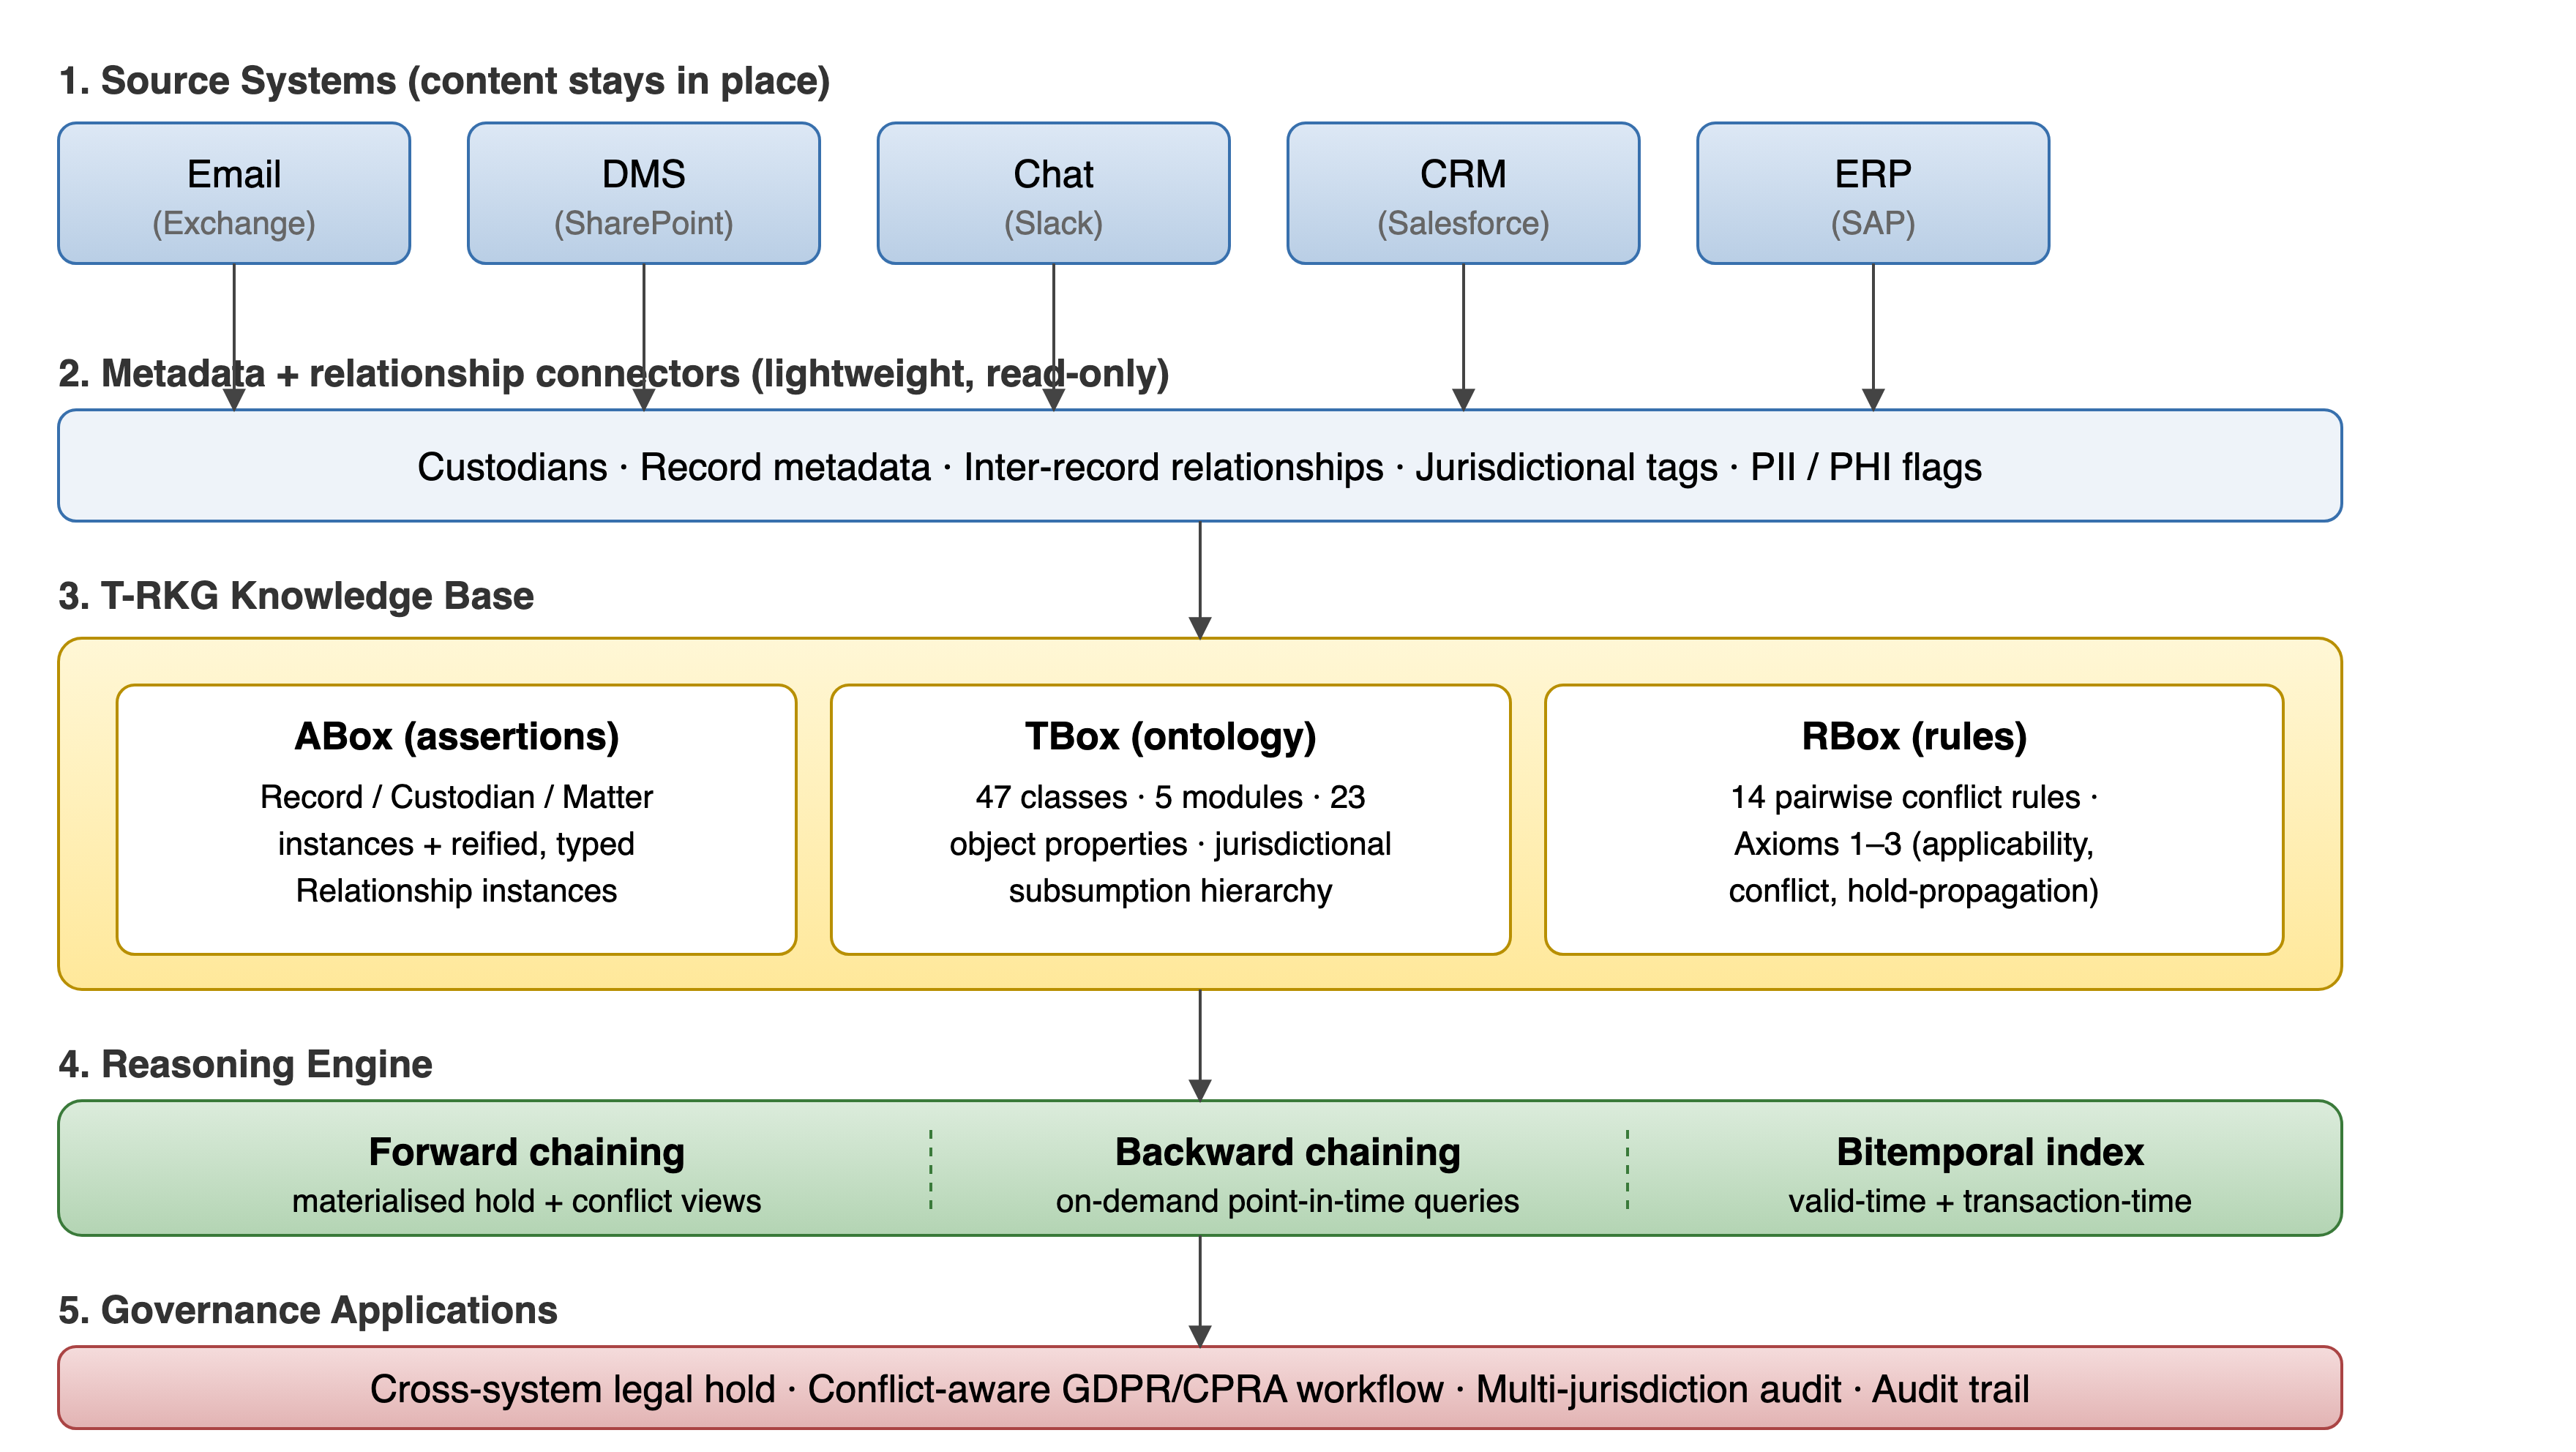
\includegraphics[width=\linewidth]{figures/figure1_architecture.png}
\caption{T-RKG system architecture. Source-system content remains in place. Metadata and relationship structure are extracted via the connector layer. The ontology (TBox) and rules (RBox) live in the reasoning engine. Forward chaining materializes hold and conflict views; backward chaining answers point-in-time queries.}
\label{fig:architecture}
\end{figure}

\subsection{Hold Propagation}

Propagation is a typed BFS (Algorithm~\ref{alg:propagation}): at each edge in the frontier, the \textsc{ShouldPropagate} function consults the ontology for the relationship type's \texttt{propagatesHold} value and evaluates the current matter's propagation policy. Four propagation policies are predefined: Conservative (attachment and thread relationships only), Standard (adding derivation relationships), Comprehensive (all typed relationship classes), and Custom. The Conservative default is the smallest scope that preserves attachments and threads — the relationship types whose loss would be hardest to defend in a preservation challenge. Validity-interval intersection between the relationship's $[t_s, t_e]$ and the matter's active interval is currently performed by the connector layer when relationships are extracted, not inside \textsc{ShouldPropagate}; folding the Allen-style~\cite{allen1983} check into the propagation loop is bounded extension work.

\begin{algorithm}[t]
\caption{Semantic Hold Propagation}
\label{alg:propagation}
\begin{algorithmic}[1]
\Require Seed records $S_0$, propagation config $P$, ontology $O$, max depth $d$
\Ensure Hold set $H$
\State $H \gets S_0$;\ \ frontier $\gets S_0$;\ \ depth $\gets 0$
\While{frontier $\neq \emptyset$ and ($d = -1$ or depth $< d$)}
    \State next $\gets \emptyset$
    \For{each $r \in$ frontier}
        \State rels $\gets$ \textsc{GetRelationships}($r$, $O$)
        \For{each $(r, r', \rho, [t_s, t_e]) \in$ rels}
            \If{\textsc{ShouldPropagate}($\rho$, $P$, $O$) and $r' \notin H$}
                \State next $\gets$ next $\cup\ \{r'\}$
            \EndIf
        \EndFor
    \EndFor
    \State $H \gets H \cup$ next;\ \ frontier $\gets$ next;\ \ depth $\gets$ depth $+ 1$
\EndWhile
\State \Return $H$
\end{algorithmic}
\end{algorithm}

\subsection{Conflict Detection}

For each record, the first stage of conflict detection is applicability reasoning via Axiom~1. The detector then evaluates fourteen pairwise conflict rules over all unordered pairs in $\mathrm{applicable}(r)$ (Algorithm~\ref{alg:conflict}): fourteen over regulation pairs, plus one Hold--Deletion rule evaluated only when an active hold is present. The fifteen rules distribute as follows: seven Retention--Deletion rules (GDPR vs.\ SOX, GDPR vs.\ HIPAA, GDPR vs.\ HGB, CPRA vs.\ SOX, CPRA vs.\ SEC, CPRA vs.\ IRS, PIPEDA vs.\ SOX); five Priority rules (SOX vs.\ SEC, SOX vs.\ IRS, SOX vs.\ HGB, SEC vs.\ IRS, HIPAA vs.\ IRS); two Jurisdiction rules (GDPR vs.\ CPRA, GDPR vs.\ PIPEDA); and one Hold--Deletion rule (active hold vs.\ GDPR Article~17 erasure). The Priority family's lex-superior / lex-specialis / lex-posterior structure follows the precedence pattern of defeasible deontic logic~\cite{governatori2013}. Severity assessment and resolution guidance are encoded in the ontology for each pair; conflict counts reported in Table~\ref{tab:conflicts} are deduplicated unordered pairs.

\begin{algorithm}[t]
\caption{Conflict Detection}
\label{alg:conflict}
\begin{algorithmic}[1]
\Require Record set $R$, ontology $O$, regulation profiles $\Pi$
\Ensure Conflict set Conflicts
\State Conflicts $\gets \emptyset$
\For{each $r \in R$}
    \State applicable $\gets$ \textsc{InferApplicable}($r$, $\Pi$, $O$)
    \For{each unordered pair $\{\gamma_1, \gamma_2\} \subseteq$ applicable, $\gamma_1 \neq \gamma_2$}
        \If{$\mathrm{conflictsWith}(\gamma_1, \gamma_2) \in \Pi$}
            \State type $\gets$ \textsc{ClassifyConflict}($\gamma_1, \gamma_2$, $O$)
            \State sev $\gets$ \textsc{AssessSeverity}($\gamma_1, \gamma_2$, $r$, $O$)
            \State guidance $\gets$ \textsc{ResolveGuidance}($\gamma_1, \gamma_2$, $O$)
            \State Conflicts $\gets$ Conflicts $\cup\ \{(r, \gamma_1, \gamma_2, \mathrm{type}, \mathrm{sev}, \mathrm{guidance})\}$
        \EndIf
    \EndFor
\EndFor
\State \Return Conflicts
\end{algorithmic}
\end{algorithm}

\subsection{A Worked Trace}

Consider record \texttt{fin\_00112} generated under seed 42 with attributes: type = Invoice, jurisdiction = EU\_DE, contains\_pii = True, metadata.is\_public\_company = True (verified against the supplementary store at \texttt{generate\_store(10000, seed=42).records['fin\_00112']}). The detector executes four steps. Step~1 (Axiom~1, jurisdiction subsumption): the record's ancestor jurisdictions are $\{\mathrm{EU\_DE, EU, GLOBAL}\}$. Each regulation profile's \texttt{appliesIn} set is intersected against this; record-type and attribute conditions are then evaluated. Step~2 (applicable regulations): $\mathrm{applicable}(r) = \{\mathrm{GDPR, SOX, HGB}\}$. Step~3 (Axiom~2, pairwise conflict check over unordered pairs): three lookups in the conflict-rule table yield (GDPR, SOX) $\rightarrow$ RetentionDeletion CRITICAL; (GDPR, HGB) $\rightarrow$ RetentionDeletion HIGH; (SOX, HGB) $\rightarrow$ Priority MEDIUM. Step~4 (resolution guidance): each conflict carries the ontology-attached resolution string.

\textbf{Exemption branch (Axiom~4).} If the same record is later placed under a legal hold for a litigation matter $m$ whose \texttt{legalClaim} flag is set (for example, a customer dispute on the underlying invoice), the detector runs one extra step before emitting any Hold-Deletion conflict. With \texttt{legalClaim}$(m){=}\mathrm{True}$, the Hold-vs-GDPR conflict that Axiom~2 would have produced is suppressed and the detector's \texttt{suppressed\_exemption\_count} is incremented. The retention-deletion conflicts from Step~3 are unaffected: the exemption is scoped to the Hold-Deletion pair, matching the structure of the GDPR text. Running the supplementary code reproduces the trace step by step.

\subsection{Temporal Query Answering}

The data model accommodates bitemporal modeling via two orthogonal time axes~\cite{snodgrass1995,jensen1997}; the present evaluation exercises only the valid-time axis (a transaction-time experiment is roadmap work, §VIII-E). The two axes are: valid time captures when a relationship or governance state held in the external world; transaction time records when that state was first registered in the system. Propagation and conflict queries can be evaluated at any valid-time point $t$, enabling retrospective hold reconstruction. The current evaluation in §VII exercises valid-time queries; a transaction-time experiment (two-wave ingestion with corrected timestamps) is the next item on the evaluation roadmap.

\subsection{Complexity and Soundness}

We state the operational properties of the reasoning machinery formally. Let $n = |R|$, $m = |E|$, and $\gamma = |\Gamma|$ (the number of encoded regulations).

\begin{proposition}[Conflict-detection complexity]
Algorithm~\ref{alg:conflict} runs in time $O(n \cdot \gamma^2)$ under the assumption that applicability evaluation per profile is $O(1)$ and conflict-rule lookup is $O(1)$ via a precomputed table.
\end{proposition}

\begin{proof}[Proof sketch]
The outer loop iterates $n$ records. For each record the applicability pass is $O(\gamma)$. The unordered pairwise conflict check enumerates pairs of applicable regulations, bounded above by $\binom{\gamma}{2} \leq \gamma(\gamma-1)/2$. With $\gamma \leq 9$ in the current implementation, the per-record cost is bounded by 36 lookups. The empirical scaling reported in §\ref{sec:scalability} ($\approx 3.3$~ms per 1{,}000 records, linear through 100K) is consistent with this bound.
\end{proof}

\begin{proposition}[Propagation complexity]
Algorithm~\ref{alg:propagation} runs in time $O(|H| + |E_H|)$ where $E_H \subseteq E$ is the set of edges incident to records reached during the traversal, restricted to relationship types $\rho$ for which $\textsc{ShouldPropagate}(\rho, P, O)$ holds.
\end{proposition}

\begin{proof}[Proof sketch]
BFS visits each reached node once and each incident edge once; the policy filter $\textsc{ShouldPropagate}$ is an $O(1)$ ontology lookup per edge. Edge-type filtering reduces $|E_H|$ by the per-policy-included fraction.
\end{proof}

\begin{proposition}[Soundness of Axiom~3]
Let $H_{P,d}(S_0)$ denote the hold set computed by Algorithm~\ref{alg:propagation} on seeds $S_0$ under policy $P$ at depth $d$. Then for every $r \in H_{P,d}(S_0)$ there exists a typed-relationship path $r_0 \to r_1 \to \cdots \to r_\ell = r$ of length $\ell \leq d$ such that $r_0 \in S_0$ and $\mathrm{propagatesHold}(\rho_i)$ holds under $P$ for every edge in the path.
\end{proposition}

\begin{proof}
By induction on the depth at which $r$ enters $H$. Base: at depth 0 only seeds enter; the empty path satisfies the claim trivially. Step: a node $r$ enters at depth $\ell + 1$ only via line~7 of Algorithm~\ref{alg:propagation}, which requires an edge $(r', r, \rho)$ with $r' \in$ frontier (so $r'$ entered at depth $\leq \ell$, with a witnessing path $\pi'$ by induction) and $\textsc{ShouldPropagate}(\rho, P, O)$. The path $\pi'$ followed by $(r', r, \rho)$ is the witnessing path for $r$.
\end{proof}

Proposition~4 (recall ceiling for the No-Ontology baseline) and Corollary~1 (zero cross-domain detection under attribute-blind tagging) are stated in §VII-D, where they sit adjacent to the capability-ablation numbers they explain.

\section{Implementation}

\subsection{Technology Choices}

The prototype is implemented in Python, using NetworkX~\cite{networkx} for in-memory graph storage and traversal. Records are stored as typed nodes. Relationships are stored as directed, labeled edges with temporal attributes and semantic property annotations. Four dedicated entity indices (by record type, by custodian, by jurisdiction, and by hold membership) support the $O(1)$ lookup patterns that governance operations invoke most frequently. NetworkX was selected for transparency. A production deployment at the scale of millions of records would benefit from a native graph database backend (Neo4j, Amazon Neptune, JanusGraph). The linear scaling observed in these experiments is consistent with such a migration being feasible. This remains a limitation acknowledged in §VIII-E.

\subsection{Regulation Profiles}

Each of the nine encoded regulations is specified as a profile with five components: (i)~applicable record-type classes; (ii)~jurisdictional scope, resolved against the hierarchy; (iii)~attribute conditions on the record; (iv)~organizational metadata conditions; (v)~operative requirements with type and parameters. Adding a new regulatory framework requires authoring one profile and encoding pairwise conflict rules against the existing set. To illustrate the marginal cost: CCPA, whose applicability conditions are largely subsumed by CPRA (already in the encoded set), would require $\sim$50 lines of configuration, whereas GDPR, whose applicability involves data-subject residence conditions and several articulated exemptions, required $\sim$200 lines.

\subsection{Baseline Implementations}

Three classes of comparison baseline are used. Two test capability and isolate distinct ontological contributions. The third tests implementation performance.

The \textit{Siloed} baseline iterates every record using only the regulation set its source system would normally enforce. Per-system applicability uses the same RegulationProfile evaluator T-RKG uses. What changes is the scope of regulations the baseline is permitted to test against. This baseline detects within-system priority conflicts (e.g., SOX vs.\ SEC inside the ERP) but cannot detect any cross-domain conflict --- the structural reason is Corollary~1.

The \textit{No-Ontology} baseline constructs a unified record graph and assigns regulations from a coarse type-and-system map. Lacking PII inference, jurisdiction subsumption, and metadata reasoning, it triggers many false-positive priority conflicts and zero true cross-domain conflicts.

The \textit{performance} baselines, used only in Table~\ref{tab:perf}, are FlatListStore (records and relationships in plain Python lists with linear-scan traversal) and SQLiteStore (records and relationships in a relational database with indices and a recursive-CTE traversal). They test the storage and traversal layer. They are not graph databases, and the comparison should be read as ``T-RKG vs.\ relational and naive-list alternatives'', not against a production graph DB.

\textit{SHACL Core baseline.} A fourth capability baseline runs the same dataset through a SHACL Core validator (\texttt{pyshacl}, no SHACL-SPARQL extension). The implementation (\texttt{trkg/baselines/shacl\_baseline.py}) materializes the synthetic ABox as an RDF graph and applies two SHACL Node Shapes covering the static-constraint surface of the conflict families: one for the mutual exclusion of \texttt{governance\_state{=}DELETED} with an active \texttt{onHoldFor} link, and one for the attribute conjunction (PII, public-company, EU jurisdiction) that triggers GDPR-vs-SOX RetentionDeletion. The shape set is deliberately small: the comparison is intended to characterize the SHACL Core expressivity ceiling, not to maximize a violation count.

Four rule families fall outside that ceiling, each for a documented reason. \emph{Temporal interval intersection} requires interval algebra that SHACL Core does not provide (\texttt{sh:lessThan} compares property pairs on a single focus node). \emph{Defeasible priority resolution} requires exceptions among constraints; SHACL evaluates shapes independently. \emph{Cross-record propagation closure} requires the fixed-point semantics SHACL Core does not include. \emph{Art.~17(3) exemption suppression} requires a cross-record dependency that lifts the baseline into SHACL-SPARQL. These limitations are catalogued in \texttt{shacl\_limitations.json}. At 100K records, the baseline detects $280 \pm 38$ violations against T-RKG's $7{,}610 \pm 303$, and takes $20{,}347 \pm 261$~ms against $326 \pm 14$~ms for T-RKG. The full per-scale comparison appears in §VII-C.

\subsection{The Cross-System Attribute Partition}
\label{sec:partition}

Two of the experiments below---the composition ablation (§\ref{sec:composition}) and the LLM baseline (§\ref{sec:llm})---require a faithful model of which source system natively holds which attribute, so that a ``siloed'' view can be constructed. Each governance-relevant attribute is assigned a single canonical home system reflecting typical enterprise system-of-record ownership: personally identifiable and health information are mastered in the customer-relationship system (CRM); public-company/listing status in the financial system of record (ERP); while jurisdiction and record type are intrinsic to each record and always visible. The siloed view of a record retains only the attributes whose home system equals the record's own source system $\sigma(r)$ and masks every foreign attribute, making cross-system composition an explicit, switchable variable. The partition is enforced at runtime: an assertion fails loudly if any siloed view still exposes a foreign attribute, so a leaking partition cannot silently inflate a result.

Two properties of this map are worth stating, because both bear on how the siloed results should be read. First, the single-canonical-home assignment is a deliberate \emph{idealization}: in practice PII is scattered across many systems (HR, email, CRM, data lakes), not single-homed. This idealization is conservative against our own thesis---it gives the siloed baseline the most favorable possible partition (clean, non-overlapping, maximally coherent), so the cross-domain collapse it nonetheless exhibits is a \emph{lower bound} on the fragmentation a real, more scattered enterprise would impose. Second, the PHI$\rightarrow$CRM and public-company$\rightarrow$ERP assignments are modeling stand-ins (PHI would more naturally live in a clinical or EHR system, listing status in a reference/MDM system); folding them into CRM and ERP keeps the five-system model tractable, and the experiment depends only on the soundness of the partition (no attribute has two homes), not on the specific vendor assignment.

\section{Evaluation}
\label{sec:eval}

The evaluation begins with the substantive accuracy claim. §VII-B reports per-record applicability F1 against a held-out clean-label snapshot of the regulation-assignment function, in clean and noised regimes; this measures the robustness of applicability reasoning under input corruption rather than agreement with an external legal standard (§VIII-E discusses an independent-expert validation of the encoded predicate). §VII-C extends the comparison to a SHACL Core baseline --- the strongest expressive baseline within standard RDF validation --- and then to a SHACL-SPARQL baseline (§\ref{sec:shaclsparql}). §\ref{sec:llm} reports an LLM applicability baseline that isolates cross-system composition as the operative difficulty. §VII-D then reports conflict counts at scale and frames them as a capability ablation: by Corollary~1, the attribute-blind baselines cannot detect cross-domain conflicts in principle, so the ``0~$\pm$~0'' columns are predictions of the proof rather than independent measurements; §\ref{sec:composition} ablates composition empirically. The remaining subsections cover hold-propagation coverage and the contribution of individual relationship types (§VII-E), scalability and matter-scoped latency (§VII-F), three end-to-end governance scenarios (§VII-G), the relationship-type ablation (§VII-H), implementation-layer performance against flat-list and SQLite baselines (§VII-I), propagation latency vs.\ seed-set size (§VII-J), the Art.~17(3) exemption-impact experiment (§VII-K), a parameter-sweep robustness experiment (§VII-L), and the reproduction recipe (§VII-M).

We state plainly which results carry the empirical weight, because two of the comparisons in this section are honest disclaimers rather than measurements: the clean-regime F1 of 1.000 is a definitional identity, and the zero cross-domain counts of the attribute-blind baselines are forced by Corollary~1. The contribution does not rest on either. It rests on three results that are not true by construction: (i) the composition ablation (§\ref{sec:composition}), where removing cross-system composition---with the ontology and regulation set held fixed---collapses cross-domain detection to zero on every seed; (ii) applicability robustness under 10\% attribute noise (§\ref{sec:f1}), where T-RKG attains F1 $0.826 \pm 0.011$ and separates from both baselines at the significance floor; and (iii) the expressivity ceiling of standards-based validation (§\ref{sec:shacl}, §\ref{sec:shaclsparql}) and of a prompted LLM denied the composed record (§\ref{sec:llm}). The disclaimers are stated for rigor; these three are the evidence.

\subsection{Experimental Setup}

\textbf{Compute environment.} All measurements taken on a single workstation: Apple~M4 system-on-chip, 10~CPU~cores (4~performance + 6~efficiency), 16~GB unified memory, NVMe SSD, macOS~15.6.1 (Darwin 24.6.0), CPython 3.12.12, NetworkX 3.x, tracemalloc from CPython 3.12. All experiments run single-process, single-thread. Wall-clock times via \texttt{time.perf\_counter()}. Memory measurements use \texttt{tracemalloc}, which adds a known 20\% to 30\% overhead documented by the CPython performance team.

\textbf{Data generation.} All evaluation data are synthetically generated. Six dataset sizes: 1K, 5K, 10K, 25K, 50K, 100K records. Content-type proportions — email (40\%), documents (30\%), chat (15\%), contracts (5\%), financial records (5\%), tickets (5\%) — are a plausible enterprise prior rather than a measured industry distribution; the parameter-sweep in §VII-L examines how conflict counts move under variations of the two parameters (EU jurisdictional fraction and PII rate) that should matter most for the conflict-detection workload.

\textbf{Statistical methodology.} All experiments are replicated across ten random seeds (42, 123, 456, 789, 1024, 2026, 31415, 65537, 1729, 2718). Results are reported as mean $\pm \sigma$. For paired comparisons across systems a paired permutation test on the per-seed differences is reported, with 10{,}000 sign-flip resamples; with $n{=}10$ the resolvable two-sided $p$-floor sits at $2/2^{10} \approx 0.002$, well below the conventional $\alpha=0.05$ threshold. T-RKG dominates Siloed on cross-domain conflicts across all ten seeds at every scale in Table~\ref{tab:conflicts}, attaining this floor uniformly. Cohen's $d$ is reported alongside as an effect-size context. Where a baseline's logic is deterministic per record type (so $\sigma=0$ across all seeds and the rank statistic is undefined), the corresponding cells are marked ``(det.)'' in the table and explained in the caption. Where the resolvable floor is structurally insufficient (the Art.~17(3) suppression-rate estimation in §VII-K, where the per-seed exemption count has a discrete distribution because exemption flags are sampled at $p{=}0.05$ on a five-matter population), the variance column is reported as-is and treated as an artifact of the sampling design rather than a quantity to be tightened by re-running. Every reported number is produced by the single orchestration script \texttt{experiments/run\_all.py}.

\subsection{Applicability F1 in Two Regimes --- Headline Result}
\label{sec:f1}

The substantive accuracy claim is per-record regulatory applicability under realistic input corruption. Table~\ref{tab:f1noise} reports F1 across three systems on a 10K-record corpus with 10\% i.i.d.\ label noise injected independently across the PII, jurisdiction, and public-company attributes after a clean-label snapshot. T-RKG achieves F1 of $0.826 \pm 0.011$, a 22-point gap over the Siloed baseline ($0.604 \pm 0.035$) and a 69-point gap over the No-Ontology baseline ($0.141 \pm 0.011$). The No-Ontology recall ceiling of 0.491 is the empirical realization of Proposition~4 (stated in §VII-D, where it is positioned next to the capability-ablation numbers it explains). We state the scope of this result plainly: the snapshot is the regulation-assignment function's own clean-label output, so the experiment measures how well T-RKG's reasoning degrades under attribute corruption, not agreement with an external legal authority; §VIII-E reports a separate independent-expert validation of the encoded applicability predicate.

Two regimes are reported. In the clean regime (Table~\ref{tab:f1clean}), the generator produces records and the system must recover the regulation set the ontology assigns under their clean attributes. T-RKG's applicability predicate coincides with the generator's regulation-assignment function on clean inputs, so its F1 on this regime is a definitional identity (1.000) and is omitted from the table; the rows of value are No-Ontology and Siloed, which quantify the gap each baseline incurs against the ontological reference. In the noised regime (Table~\ref{tab:f1noise}), 10\% per-attribute label noise is injected after the ground-truth labels are snapshotted: 10\% of jurisdictions are flipped to a random alternative, 10\% of PII flags are flipped, and 10\% of public-company flags are flipped. The system must reason from possibly-corrupted attributes back to the underlying truth.

\begin{table}[t]
\centering
\caption{Per-record applicability, clean regime (10K dataset, 10 seeds). T-RKG matches the ontological reference predicate by construction; the table reports the baseline gap.}
\label{tab:f1clean}
\begin{tabular}{lccc}
\hline\hline
System & Precision & Recall & F1 \\
\hline
No-Ontology       & $0.083 \pm 0.007$ & $0.491 \pm 0.033$ & $0.141 \pm 0.011$ \\
Siloed            & $1.000 \pm 0.000$ & $0.491 \pm 0.033$ & $0.657 \pm 0.032$ \\
\hline\hline
\end{tabular}
\end{table}

\begin{table}[t]
\centering
\caption{Per-record applicability, noised regime (10\% jurisdiction + 10\% PII + 10\% public-company-flag noise, independent; 10 seeds).}
\label{tab:f1noise}
\begin{tabular}{lccc}
\hline\hline
System & Precision & Recall & F1 \\
\hline
T-RKG       & $0.790 \pm 0.018$ & $0.864 \pm 0.005$ & $0.826 \pm 0.011$ \\
No-Ontology & $0.083 \pm 0.007$ & $0.491 \pm 0.033$ & $0.141 \pm 0.011$ \\
Siloed      & $0.991 \pm 0.006$ & $0.435 \pm 0.028$ & $0.604 \pm 0.035$ \\
\hline\hline
\end{tabular}
\end{table}

\begin{figure}[t]
\centering
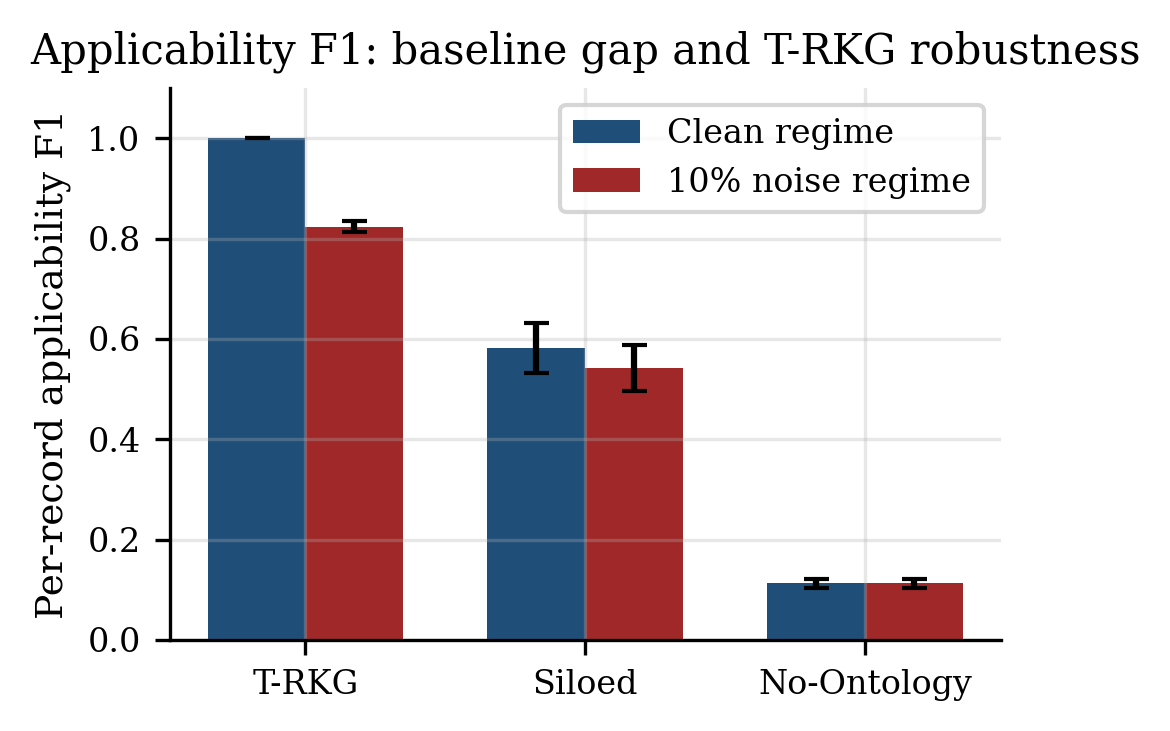
\includegraphics[width=\linewidth]{figures/fig5_f1_clean_vs_noise.png}
\caption{Per-record applicability F1 in the clean and noised regimes. Error bars are $\pm \sigma$ across 10 seeds.}
\label{fig:f1}
\end{figure}

Under the noised regime T-RKG loses approximately 17 F1 points. This loss is what rules out circularity: were the clean-regime F1 of 1.000 merely a tautology of the generator's labeling scheme, perturbing the labels would leave the score untouched. The T-RKG advantage over both baselines in the noised regime is significant under the paired permutation test, at the $n{=}10$ two-sided floor ($p = 0.00195$) with large paired effect sizes: $d = 7.1$ against the Siloed baseline and $d = 74$ against the No-Ontology baseline. The No-Ontology effect size is inflated by the near-constancy of that baseline's per-seed F1 (the paired difference has very small variance) and should be read together with the $p$-value rather than as a literal magnitude.

\textbf{Noise-rate sensitivity.} Fig.~\ref{fig:noise_sweep} reports T-RKG's per-record F1 across noise rates from 2\% to 20\% (applied simultaneously and independently to the PII, jurisdiction, and public-company attributes). T-RKG degrades smoothly from $F1 = 0.965 \pm 0.004$ at 2\% noise to $F1 = 0.672 \pm 0.018$ at 20\% noise, a gradient consistent with attribute-level redundancy in the applicability predicate (each regulation's $\phi_\gamma$ is a conjunction over multiple attributes, so the probability that any single regulation is fully corrupted scales worse than linearly in any single attribute's flip rate). The Siloed baseline degrades from $0.647 \pm 0.030$ to $0.554 \pm 0.031$ over the same range. The No-Ontology baseline is approximately flat at $0.141$: its recall is capped below the noise floor by Proposition~4 because its applicability function does not consult the corrupted attributes at all.

\begin{figure}[t]
\centering
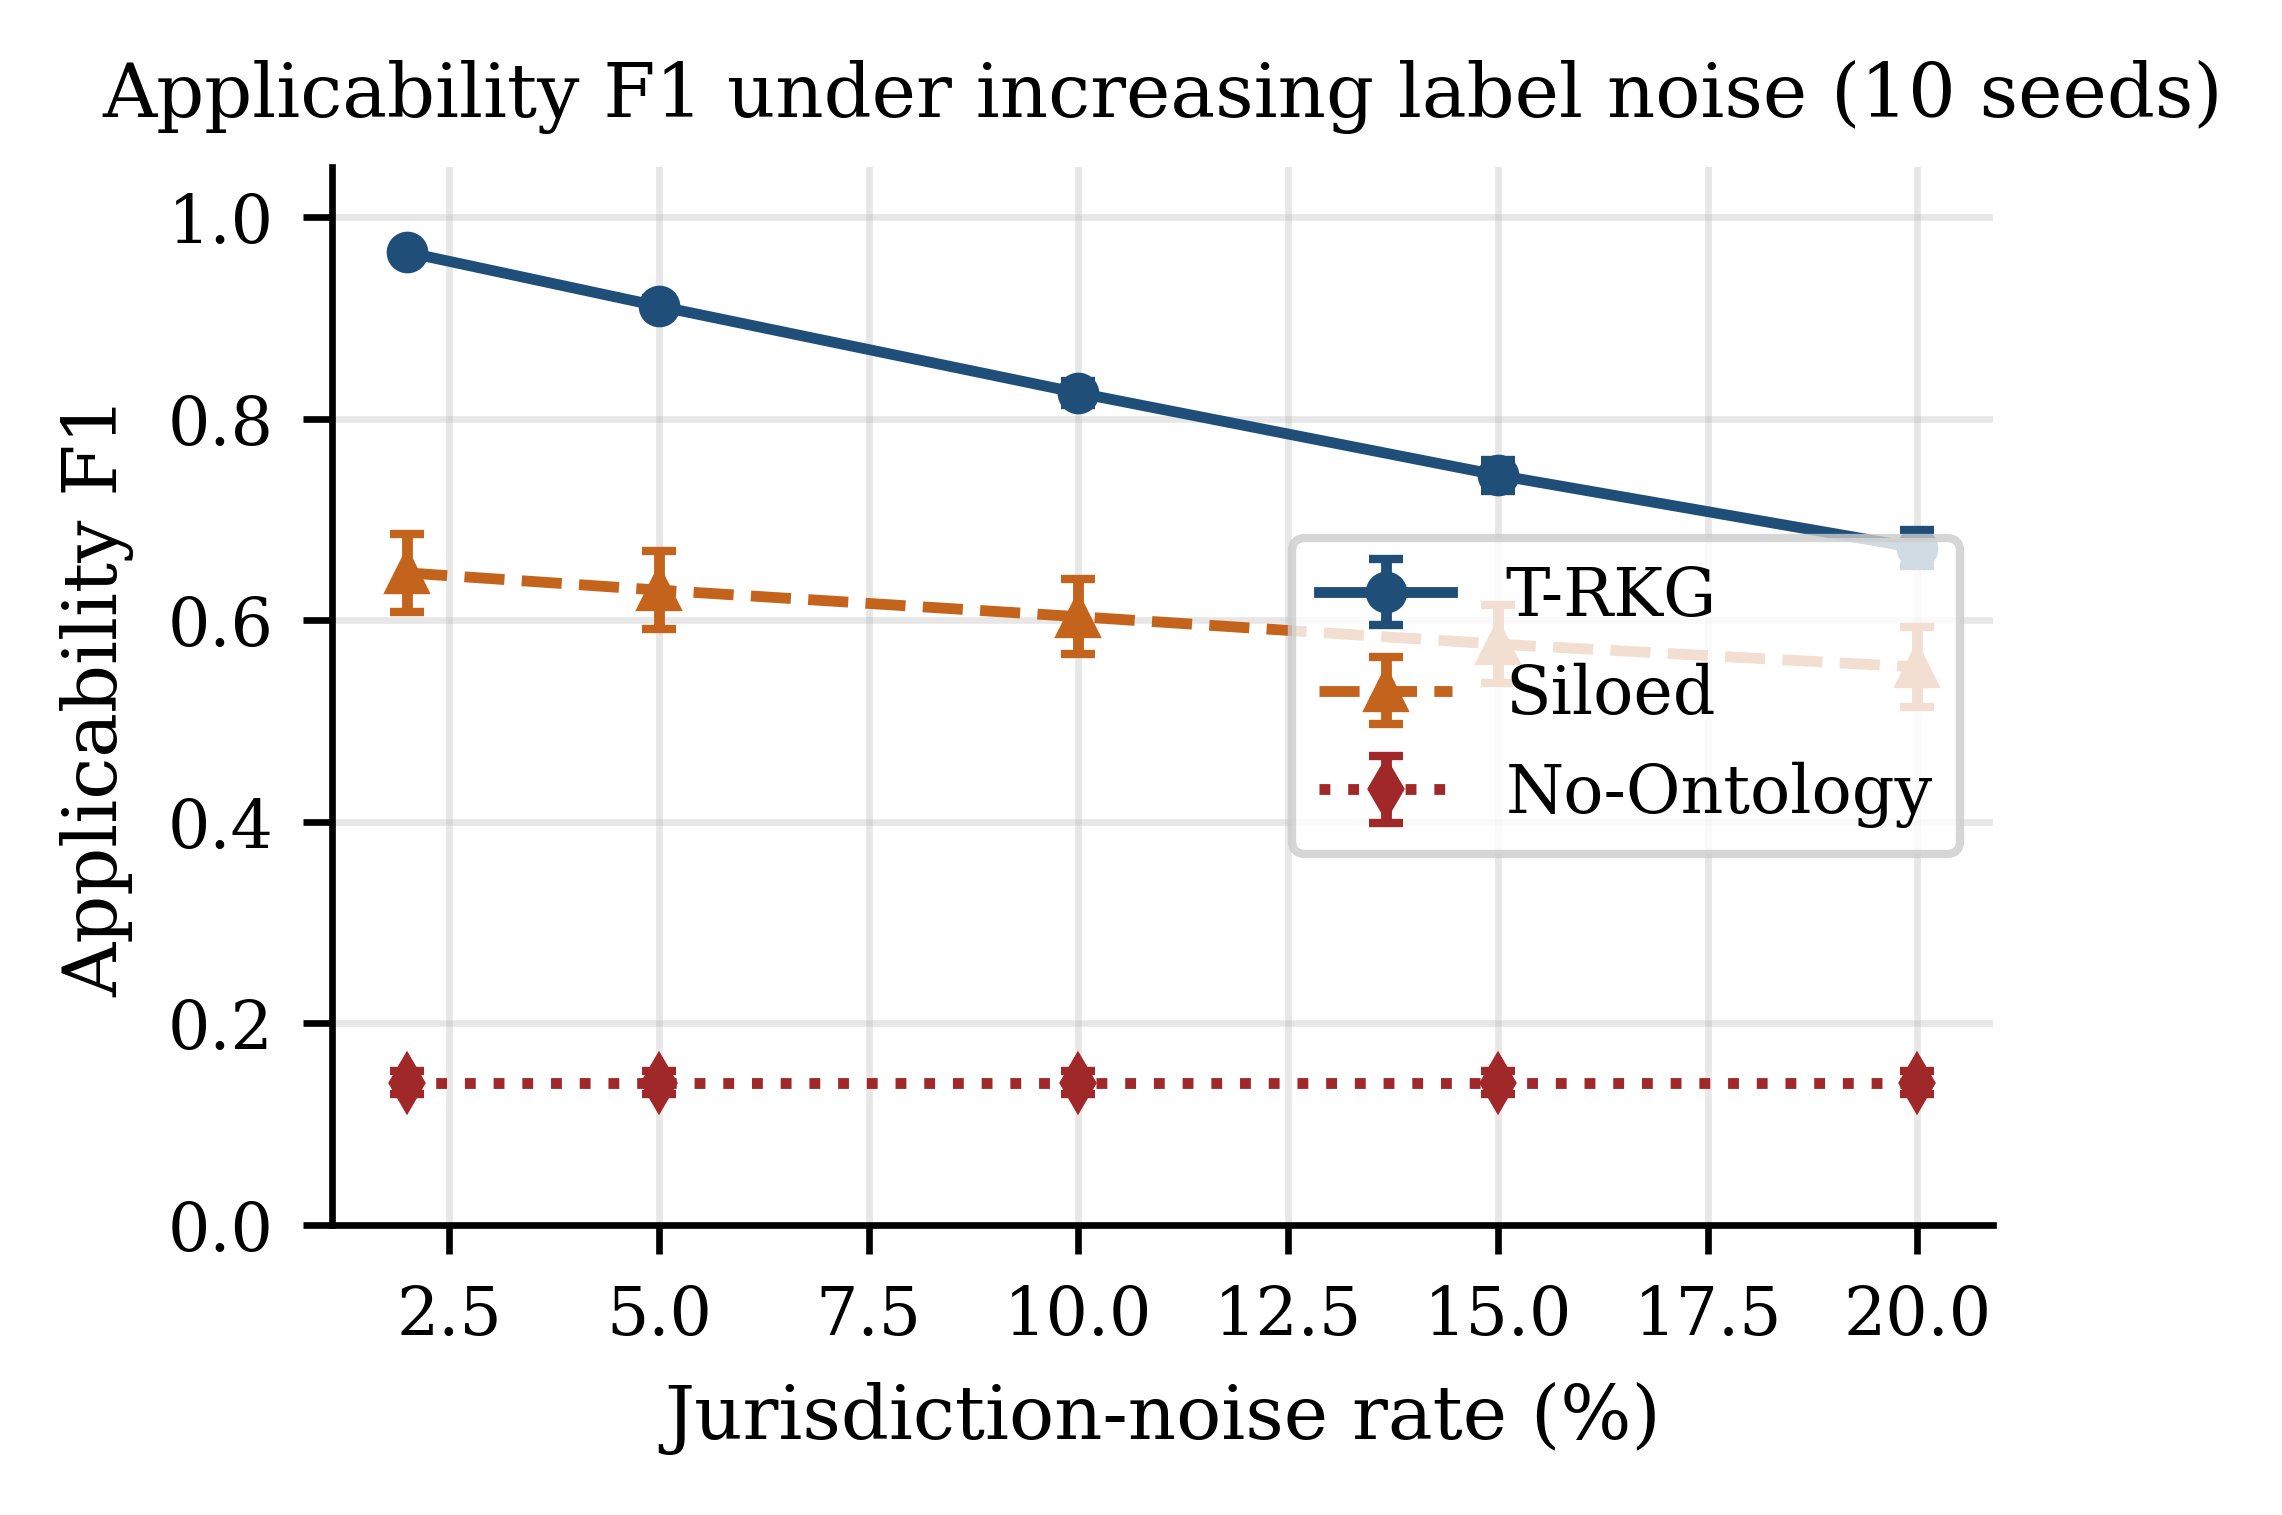
\includegraphics[width=\linewidth]{figures/fig_noise_sweep.png}
\caption{Applicability F1 vs.\ per-attribute noise rate. Error bars are $\pm \sigma$ across 10 seeds. T-RKG degrades smoothly; Siloed degrades modestly; No-Ontology is at the Proposition~4 ceiling regardless of noise rate.}
\label{fig:noise_sweep}
\end{figure}

\textbf{Block-correlated noise.} An i.i.d.\ per-attribute flip model does not represent the structure of real source-system corruption, where errors tend to be correlated (a single bad ingestion run flips an entire batch; jurisdiction confusion follows administrative geography). A companion experiment overrides the jurisdiction attribute for 10 contiguous blocks of 100 records (10\% of the corpus, matching the i.i.d. comparator's flip count on the jurisdiction attribute alone but concentrated). T-RKG attains $F1 = 0.954 \pm 0.020$ under block-correlated jurisdiction noise --- higher than the 0.826 reported above under the broader i.i.d. regime, because the broader regime corrupts all three attributes while the block experiment corrupts only one. The Siloed baseline reaches $0.648 \pm 0.032$ (similar to the clean-regime baseline ceiling, because its applicability function ignores PII and public-company anyway and is therefore insensitive to the jurisdiction-only corruption pattern when PII/public-company are clean). The No-Ontology baseline is unaffected for the same reason. The block-correlated experiment is not a substitute for production-data evaluation (§VIII-E); it is a sanity check that the i.i.d. noise model is not artificially flattering to T-RKG by spreading the same flip budget thinly across the three attributes.

The i.i.d.\ per-attribute flip model does not capture all modes of real source-system corruption --- biased missingness, jurisdictional confusion concentrated along administrative-geography boundaries, semantic confusions between adjacent regulation families are all plausible in production --- and a structured-noise regime that targets these modes is on the evaluation roadmap (§VIII-E).

\subsection{SHACL Core Comparison}
\label{sec:shacl}

Table~\ref{tab:shacl} reports the SHACL Core baseline (\texttt{pyshacl} 0.31) on the same six scales as Table~\ref{tab:conflicts}. The baseline runs two NodeShapes covering the static-constraint surface; the four out-of-scope rule families (temporal interval intersection, defeasible priority resolution, cross-record propagation closure, Art.~17(3) exemption) are catalogued in the supplementary \texttt{shacl\_limitations.json} with the SHACL feature gap responsible and the W3C-specification reference.

\begin{table}[t]
\centering
\caption{SHACL Core baseline vs.\ T-RKG (mean $\pm \sigma$ across 10 seeds). SHACL Core detects only the static-constraint subset of conflict families.}
\label{tab:shacl}
\begin{tabular}{rrrrr}
\hline\hline
Scale & SHACL viol. & SHACL (ms) & T-RKG total & T-RKG (ms) \\
\hline
1{,}000   & $2 \pm 3$    & $196 \pm 4$       & $84 \pm 16$       & $3.1 \pm 0.1$ \\
5{,}000   & $17 \pm 19$  & $1{,}018 \pm 66$  & $373 \pm 66$      & $15.6 \pm 0.2$ \\
10{,}000  & $36 \pm 27$  & $2{,}020 \pm 19$  & $740 \pm 85$      & $31.5 \pm 0.4$ \\
25{,}000  & $80 \pm 40$  & $5{,}083 \pm 46$  & $1{,}783 \pm 224$ & $79.8 \pm 2.7$ \\
50{,}000  & $165 \pm 53$ & $10{,}164 \pm 100$ & $3{,}730 \pm 330$ & $159 \pm 2$ \\
100{,}000 & $280 \pm 38$ & $20{,}347 \pm 261$ & $7{,}610 \pm 303$ & $326 \pm 14$ \\
\hline\hline
\end{tabular}
\end{table}

At 100K records, SHACL Core detects roughly 4\% of the conflicts T-RKG detects (3.7\% at 100K; about 4\% pooled across scales), and takes about $62\times$ longer to do so. The low recall is not a comparison artifact; it is what SHACL Core can do by construction. To detect temporal-interval Hold-Deletion conflicts, defeasible-priority resolutions, or hold-propagation-induced conflicts, the baseline would need SHACL-SPARQL --- which we evaluate next.

\subsection{SHACL-SPARQL Comparison}
\label{sec:shaclsparql}

SHACL Core cannot express four of the conflict families; SHACL-SPARQL (\texttt{sh:sparql} constraint components) lifts part of that ceiling by allowing SPARQL joins across nodes. We implement the conflict families as SHACL-SPARQL shapes and run them on the same balanced dataset. The result is a three-axis loss for the standards-based approach, reported as measured rather than as the anticipated ``expressivity parity at prohibitive cost.''

First, \emph{latency}. SHACL-SPARQL runs roughly $3{,}000$ to $3{,}300\times$ slower than T-RKG's native detector across the measured scales (Table~\ref{tab:shaclsparql}), peaking near $3{,}310\times$ at the smallest scale; with linear-in-$n$ scaling this projects to tens of minutes at 25K--100K records, against tens to hundreds of milliseconds for T-RKG, so the approach is infeasible at enterprise scale.

\begin{table}[t]
\centering
\caption{SHACL-SPARQL vs.\ T-RKG latency (balanced dataset, 10 seeds). Scales above 10K are projected from the measured linear fit and were not run.}
\label{tab:shaclsparql}
\begin{tabular}{rrrr}
\hline\hline
Scale & T-RKG & SHACL-SPARQL & Ratio \\
\hline
1{,}000  & 6.6~ms  & 22.0~s  & $3{,}308\times$ \\
5{,}000  & 32.6~ms & 106.3~s & $3{,}269\times$ \\
10{,}000 & 70~ms  & 215.0~s & $3{,}060\times$ \\
\hline\hline
\end{tabular}
\end{table}

Second, \emph{recall}. Even with SPARQL joins, SHACL-SPARQL reaches T-RKG's recall on only one family (Jurisdiction, $1.000$, a single uniform join); Retention--Deletion ($\sim$0.53) and Hold--Deletion ($\sim$0.46) are only partially recovered. The reason is structural rather than an implementation gap: each \texttt{sh:sparql} shape hand-encodes a single regulation pair (the Retention shape covers EU-PII $\times$ SOX public-company), so it misses CPRA/PIPEDA deletion and non-public retention; reaching T-RKG's recall would require authoring the full combinatorial cross-product of per-pair shapes by hand, which T-RKG composes automatically. The Hold--Deletion shortfall has the same character: a single defeasible shape applies the GDPR Art.~17(3) exemption uniformly across jurisdictions, whereas T-RKG fires CPRA/PIPEDA-under-hold because Art.~17(3) is GDPR-specific. (Both systems are evaluated under an identical active-hold context applied before either detector runs.)

Third, \emph{expressivity}. Priority resolution and cross-record propagation closure remain inexpressible even in SHACL-SPARQL: SHACL evaluates each shape independently and has no representation of priority among conflicting constraints, no exceptions, and no non-monotonic semantics (recall $0$ on both families). The standards-based approach therefore loses on all three axes simultaneously---partial recall absent combinatorial per-pair authoring, prohibitive latency, and families it cannot express at all.

\subsection{Why Not a Large Language Model?}
\label{sec:llm}

A natural alternative to an encoded applicability mechanism is to prompt a large language model (LLM) with a record's attributes and ask which regulations apply. We evaluate this baseline directly. A capable LLM\footnote{We use a fixed model (Claude, version pinned in the supplementary material) at temperature zero, with all responses cached; the argument is model-agnostic, since it turns on \emph{access} to attributes rather than on any model's knowledge.} is queried on a stratified sample spanning all nine regulations, in two conditions: a \emph{composed} condition in which the LLM receives the full cross-system attribute set, and a \emph{siloed} condition in which it receives only the attributes a single source system would natively hold (the partition of §\ref{sec:partition}).

The result is a sharp separation. Given the composed record, the LLM identifies applicable regulations accurately (micro-F1 $0.970$, macro-F1 $0.794$ in the clean regime); given the siloed view, its cross-domain recall collapses to $0.000 \pm 0.000$ across all ten seeds. The composed--siloed gap is large and significant (clean $\Delta = 0.721$, $p = 0.00195$, $d = 26.4$; under 10\% noise $\Delta = 0.641$, $p = 0.00195$, $d = 19.4$).

The interpretation is the central point of this subsection, and it concerns \emph{access}, not \emph{knowledge}. The LLM plainly knows the rules---its composed-condition score establishes that. What it lacks, in the siloed condition, is the assembled record: the conjunction of attributes that triggers a cross-domain conflict (e.g., a PII flag held in the customer-relationship system and a public-company flag held in the financial system of record) does not exist in any single source system, and so never reaches a model querying only that system. The composed record on which the LLM scores micro-F1 $0.970$ is an artifact that T-RKG constructs by composing attributes across silos; the LLM is excellent at the classification that remains once that composition is done, and structurally unable to perform the composition itself. Composition, not classification, is the operative difficulty, and it is what T-RKG contributes.

Two further observations sharpen the comparison. The LLM's per-regulation accuracy is uneven---near-perfect on the familiar privacy and jurisdiction rules but materially weaker on the more conditional financial regimes (e.g., IRS F1 $0.696$, HIPAA $0.886$), so the support-weighted micro-F1 of $0.970$ overstates uniform coverage; the macro-F1 of $0.794$ is the more faithful figure, and the gap between them reflects exactly the conditional, multi-attribute regulations whose applicability the LLM handles least reliably. And we note as an \emph{observation}---not as a claim of contribution, since noise-robustness is not a property T-RKG asserts---that under 10\% attribute noise the LLM's composed-condition micro-F1 ($0.872$) exceeds T-RKG's ($0.826$). This is expected and is consistent with the design: T-RKG faithfully propagates a corrupted input to a flagged output, whereas an LLM may ``reason past'' an obviously-corrupted attribute using world knowledge. For governance decisions over legal holds and erasure, that non-determinism is a liability rather than an asset---decisions must be deterministic, reproducible, and auditable to a specific rule and relationship path---and a hybrid architecture (an LLM front-end for noise-robust attribute \emph{inference} feeding T-RKG's deterministic composition and conflict layer) is a natural direction we leave to future work. The siloed collapse holds regardless: an LLM cannot detect a conflict whose triggering attributes it never sees.

\subsection{Capability Ablation: Corollary~1 in Numbers}
\label{sec:rq1}

The substantive accuracy claim is in §VII-B. This subsection isolates a separate question: when an applicability mechanism is denied the ontological attributes T-RKG consults, how many of the cross-domain conflicts surveyed in §VII-B can it still recover from a per-record-type or per-source-system tag alone? The following result formalizes why the attribute-blind baselines below cannot detect cross-domain conflicts in principle.

\begin{proposition}[Recall ceiling for the No-Ontology baseline]
Let $\Gamma_{\mathrm{PII}} \subseteq \Gamma$ be the set of regulations whose applicability profile requires the PII attribute (GDPR, CPRA, PIPEDA in the ontology). Let $\Gamma_{\mathrm{pubco}} \subseteq \Gamma$ be the set whose applicability requires the public-company organizational metadata flag (SOX, FINRA). Any baseline whose per-record regulation tagging function does not consult the PII flag (resp.\ the public-company flag) achieves zero recall on every regulation in $\Gamma_{\mathrm{PII}}$ (resp.\ $\Gamma_{\mathrm{pubco}}$) on records whose ground-truth applicability set includes the regulation only because that attribute holds.
\end{proposition}

\begin{proof}
Direct from the contrapositive of the applicability profile $\phi_\gamma$ as a conjunction over attribute predicates. If the predicate on attribute $a$ is not consulted, every record whose ground-truth applicability is conditional on $a$ is misclassified.
\end{proof}

\begin{corollary}
Any baseline whose tagging is conditioned only on (record\_type, source\_system) cannot recover regulations whose applicability is conditional on jurisdiction subsumption, PII flag, PHI flag, or organizational metadata. Cross-domain conflicts (privacy-vs-financial, or jurisdictional) are by definition conditioned on at least one such attribute. Therefore any such baseline detects zero cross-domain conflicts. The empirical ``$0 \pm 0$'' cross-domain count for both baselines reported throughout §\ref{sec:eval} is a corollary of this fact, not an experimental coincidence.
\end{corollary}

Table~\ref{tab:conflicts} reports conflict counts across six scales. The Siloed and No-Ontology columns are capability ablations, not competing implementations; their zero cross-domain count is a forced consequence of the corollary above, not an empirical finding. T-RKG's own cross-domain counts grow from $7 \pm 10$ at 1K to $994 \pm 48$ at 100K, scaling roughly linearly in the population of records that fall under two or more regulations.

\subsection{Composition Ablation}
\label{sec:composition}

Corollary~1 forces the attribute-blind baselines to zero by construction; to measure the value of cross-system composition as a controlled empirical variable rather than a proof, we ablate composition directly. The \emph{decomposed} condition runs the full T-RKG reasoner---ontology intact, full regulation set---but over records whose attributes are restricted to their home source system under the partition of §\ref{sec:partition}; the \emph{composed} condition is standard T-RKG. Everything else is held constant. On the 10K dataset across ten seeds, the composed condition detects $740 \pm 89$ total conflicts ($122 \pm 33$ cross-domain); the decomposed condition detects $618 \pm 93$ total but $0 \pm 0$ cross-domain---zero on every one of the ten seeds (paired permutation $\Delta = 122.2$, $p = 0.00195$, $d = 3.69$). The decomposed remainder ($618$) is non-zero because within-silo conflicts---chiefly intra-financial Priority conflicts that are single-system by construction---survive masking; only the cross-domain families collapse. This isolates composition as the mechanism: with the ontology and regulation set unchanged, removing cross-system attribute composition removes exactly the cross-domain conflicts and nothing else.

\begin{table*}[t]
\centering
\caption{Conflict detection results across six scales. Cross-domain (CD) = retention-deletion + jurisdiction + hold-deletion conflicts. Means $\pm \sigma$ across 10 seeds. The Siloed and No-Ontology columns are capability ablations, not competing implementations; their zero cross-domain count is forced by Corollary~1 (§VII-D), not measured. ``(det.)'' marks cells that are deterministic across all ten seeds ($\sigma{=}0$); for these cells the rank-statistic comparison is undefined, see Proposition~4 and Corollary~1 for the structural reason. The substantive accuracy comparison is the noised-regime F1 in Table~\ref{tab:f1noise}.}
\label{tab:conflicts}
\begin{tabular}{rrrrrrrr}
\hline\hline
Dataset & T-RKG total & T-RKG CD & Siloed (abl.) & Siloed CD & No-Ont (abl.) & No-Ont CD & T-RKG (ms) \\
\hline
1{,}000   & $84 \pm 16$       & $7 \pm 10$   & $75 \pm 24$       & 0 (det.) & 150 (det.) & 0 (det.) & $3.1 \pm 0.1$ \\
5{,}000   & $373 \pm 66$      & $66 \pm 27$  & $293 \pm 75$      & 0 (det.) & 750 (det.) & 0 (det.) & $15.6 \pm 0.2$ \\
10{,}000  & $740 \pm 85$      & $122 \pm 31$ & $573 \pm 101$     & 0 (det.) & 1{,}500 (det.) & 0 (det.) & $31.5 \pm 0.4$ \\
25{,}000  & $1{,}783 \pm 224$ & $258 \pm 58$ & $1{,}456 \pm 243$ & 0 (det.) & 3{,}750 (det.) & 0 (det.) & $79.8 \pm 2.7$ \\
50{,}000  & $3{,}730 \pm 330$ & $513 \pm 54$ & $3{,}062 \pm 336$ & 0 (det.) & 7{,}500 (det.) & 0 (det.) & $159 \pm 2$ \\
100{,}000 & $7{,}610 \pm 303$ & $994 \pm 48$ & $6{,}359 \pm 306$ & 0 (det.) & 15{,}000 (det.) & 0 (det.) & $326 \pm 14$ \\
\hline\hline
\end{tabular}
\end{table*}

\begin{figure}[t]
\centering
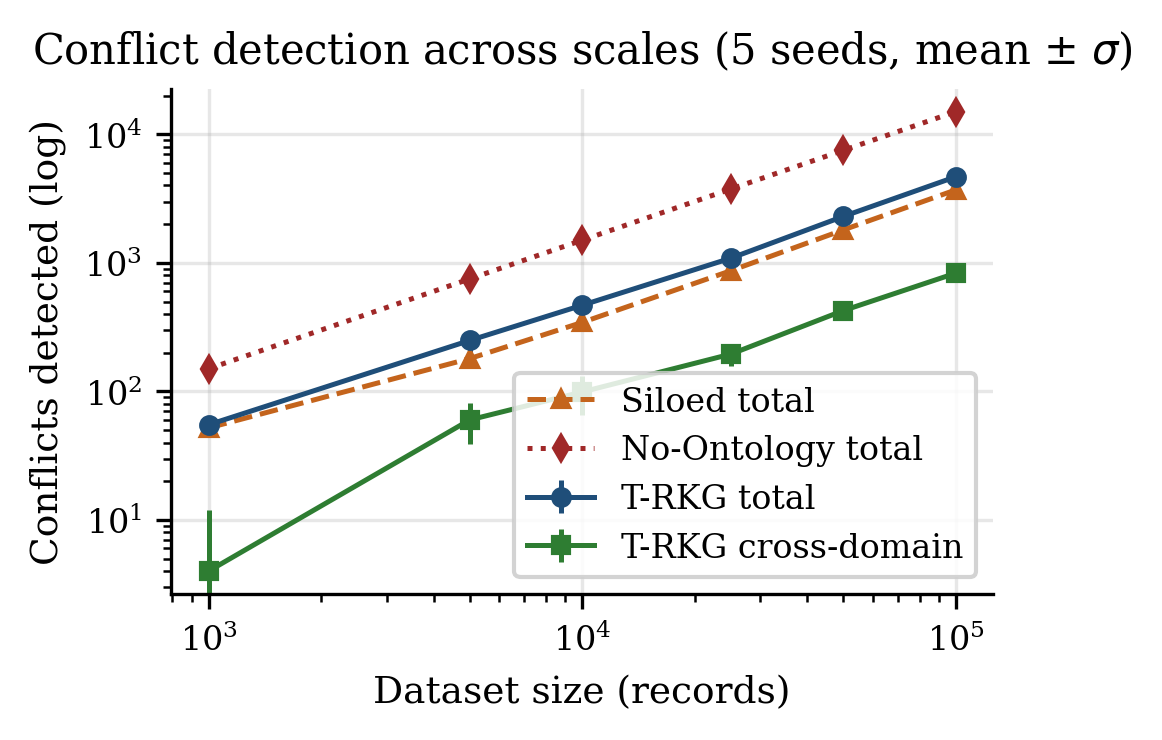
\includegraphics[width=\linewidth]{figures/fig2_conflicts_vs_scale.png}
\caption{Conflict detection counts across scales (log-log). Error bars are $\pm \sigma$ across ten seeds. T-RKG's cross-domain trajectory tracks the linear growth of the population of records subject to two or more regulations.}
\label{fig:conflicts}
\end{figure}

\begin{figure}[t]
\centering
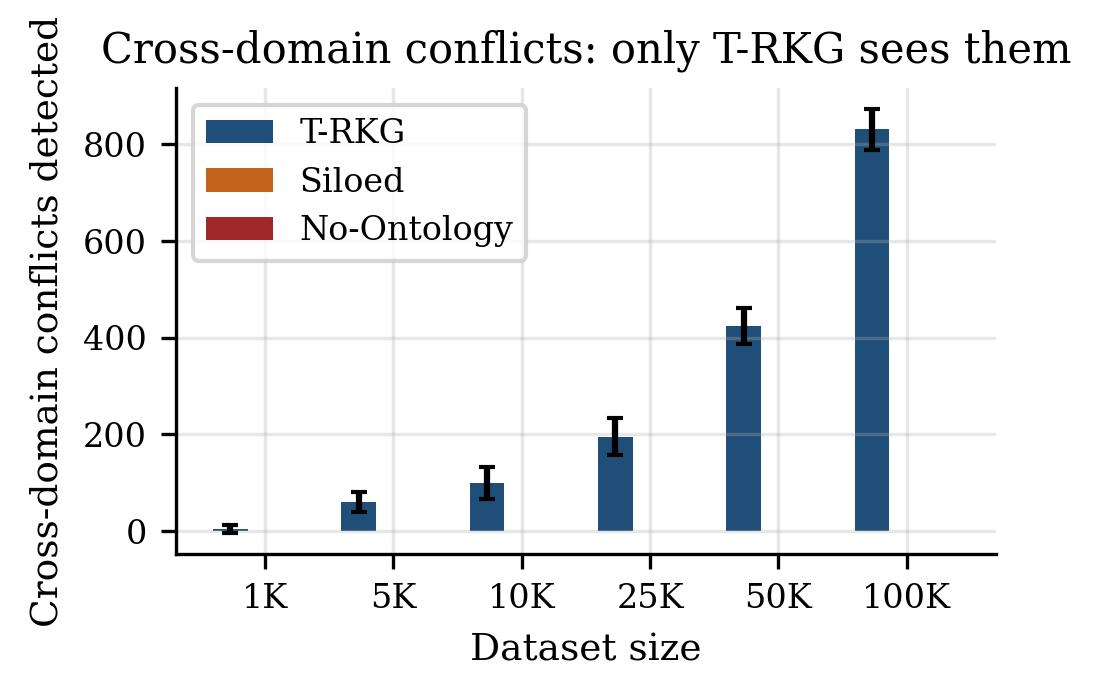
\includegraphics[width=\linewidth]{figures/fig3_cross_domain_bars.png}
\caption{Cross-domain conflicts only. Baselines return 0 by Corollary~1.}
\label{fig:crossdom}
\end{figure}

Table~\ref{tab:typesev} disaggregates the T-RKG conflicts at the 10K scale by type and severity.

\begin{table}[t]
\centering
\caption{Conflict type and severity distribution (10K dataset, 10 seeds).}
\label{tab:typesev}
\begin{tabular}{lcc}
\hline\hline
Conflict Type / Severity & Count (mean $\pm \sigma$) & \% of total \\
\hline
Retention--Deletion & $122 \pm 33$ & 16.5\% \\
Priority            & $618 \pm 93$ & 83.5\% \\
Jurisdiction        & 0            & 0\% \\
Hold--Deletion      & 0            & 0\% \\
\hline
Critical severity   & $49 \pm 25$  & 6.6\% \\
High severity       & $73 \pm 23$  & 9.9\% \\
Medium severity     & $45 \pm 35$  & 6.1\% \\
Low severity        & $573 \pm 106$ & 77.4\% \\
\hline\hline
\end{tabular}
\end{table}

Jurisdiction and Hold-Deletion conflict counts are zero at 10K because the synthetic generator at the default parameter setting produces few records whose attribute conjunctions trigger those specific rules; both rule families fire under the wider parameter sweep in §VII-L.

\subsection{RQ2 and RQ3: Hold Propagation}

Table~\ref{tab:propagation} reports propagation results for the 10K dataset, using 50 matter-scoped seed records at depth limit~10. Starting from 50 seeds, the Conservative policy (attachments and threads) produces a mean hold set of $154 \pm 52$ records, a 3.07$\times$ expansion. Adding derivation relationships increases the expansion from 3.07$\times$ to 3.30$\times$ --- a contribution that does not change the propagation-policy ordering. Expanding to all relationship types reaches 4.28$\times$, numerically close to what an untyped graph traversal would produce, with the key difference that each record in the T-RKG hold set can be traced to the specific relationship type that caused its inclusion.

\begin{table}[t]
\centering
\caption{Hold propagation by relationship configuration (10K dataset, 50 matter-scoped seed records, depth 10, 10 seeds).}
\label{tab:propagation}
\begin{tabular}{lccr}
\hline\hline
Configuration & Final Set & Ratio & Time (ms) \\
\hline
None (Siloed)   & $50 \pm 0$    & 1.00$\times$ & --- \\
Attachment      & $105 \pm 24$  & 2.11$\times$ & $0.34 \pm 0.07$ \\
Thread          & $55 \pm 5$    & 1.10$\times$ & $0.17 \pm 0.01$ \\
Att + Thread    & $154 \pm 52$  & 3.07$\times$ & $0.47 \pm 0.16$ \\
+ Derivation    & $165 \pm 55$  & 3.30$\times$ & $0.49 \pm 0.16$ \\
All types       & $214 \pm 78$  & 4.28$\times$ & $0.64 \pm 0.23$ \\
\hline\hline
\end{tabular}
\end{table}

\begin{figure}[t]
\centering
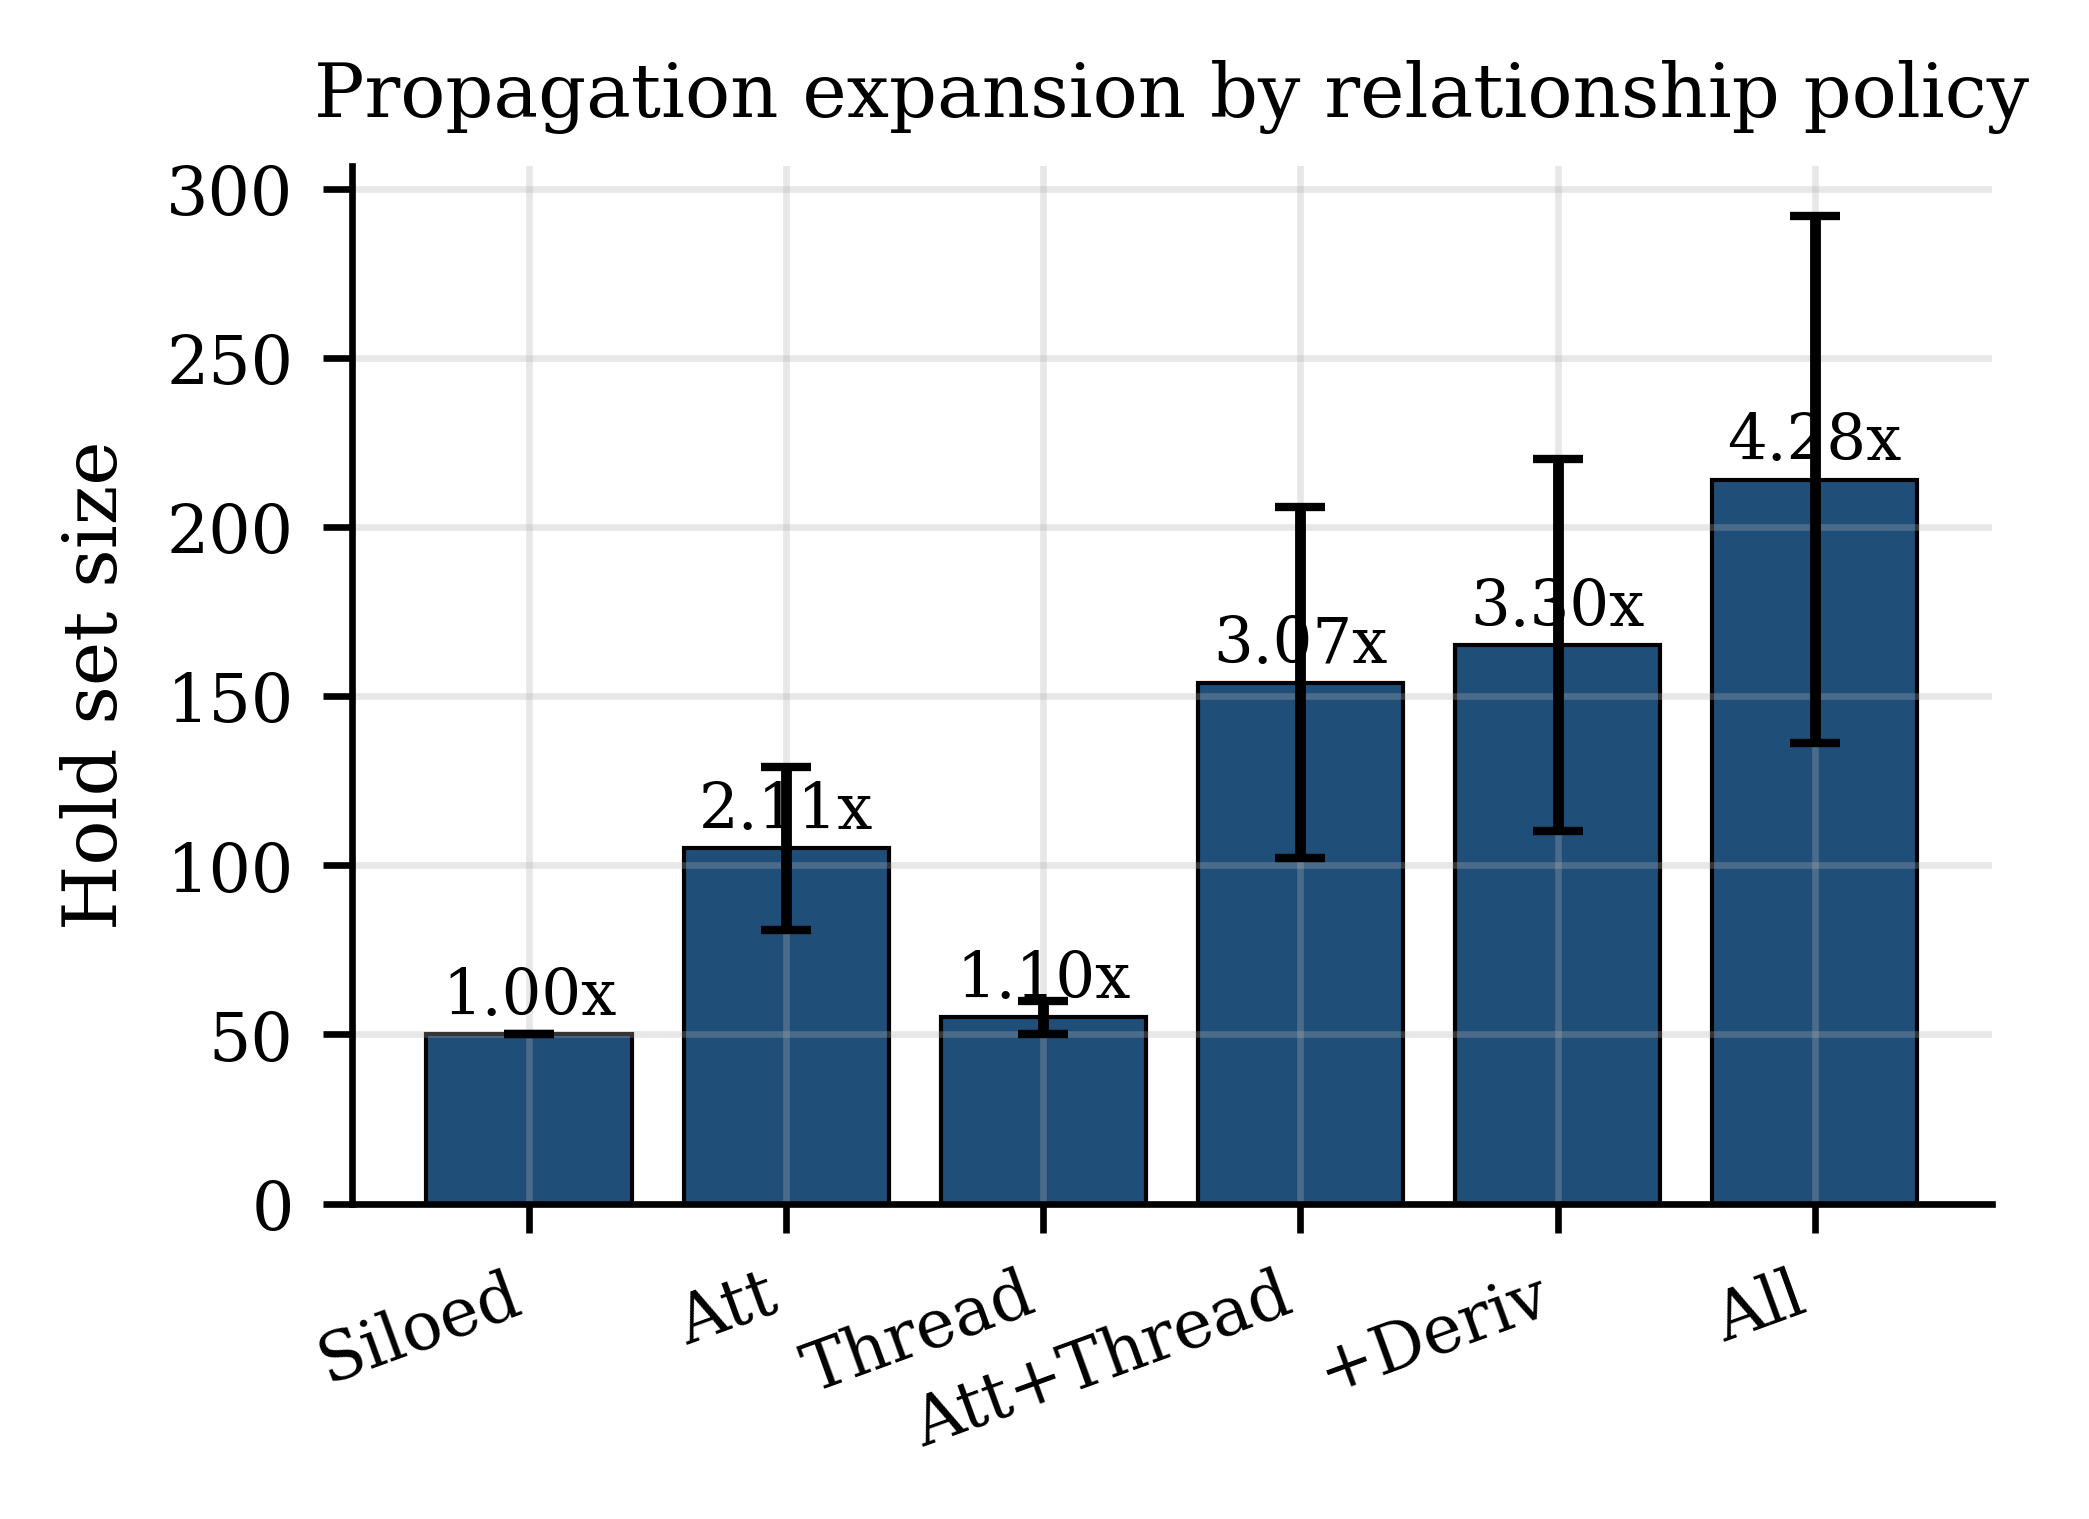
\includegraphics[width=\linewidth]{figures/fig8_propagation_policies.png}
\caption{Propagation expansion by relationship policy. Conservative (Att + Thread) yields a 3.07$\times$ expansion; the Comprehensive policy (All types) reaches 4.28$\times$ but loses the per-record relationship-type provenance.}
\label{fig:propagation}
\end{figure}

\subsection{RQ4: Scalability}
\label{sec:scalability}

\begin{table}[t]
\centering
\caption{Scalability across dataset sizes (10 seeds).}
\label{tab:scalability}
\begin{tabular}{rrrrcc}
\hline\hline
Records & Rels & Build (s) & Throughput & Prop (ms) & Mem (MB) \\
\hline
1{,}000   & 269    & 0.035 & 29{,}865/s & $0.23 \pm 0.04$ & 1.9 \\
5{,}000   & 1{,}397 & 0.174 & 28{,}999/s & $0.26 \pm 0.06$ & 9.6 \\
10{,}000  & 2{,}773 & 0.358 & 27{,}982/s & $0.27 \pm 0.08$ & 19.2 \\
25{,}000  & 6{,}935 & 0.972 & 25{,}736/s & $0.32 \pm 0.06$ & 49.6 \\
50{,}000  & 13{,}904 & 2.04 & 24{,}632/s & $0.40 \pm 0.05$ & 100.9 \\
100{,}000 & 27{,}801 & 4.10 & 24{,}432/s & $0.52 \pm 0.09$ & 198.4 \\
\hline\hline
\end{tabular}
\end{table}

\begin{figure}[t]
\centering
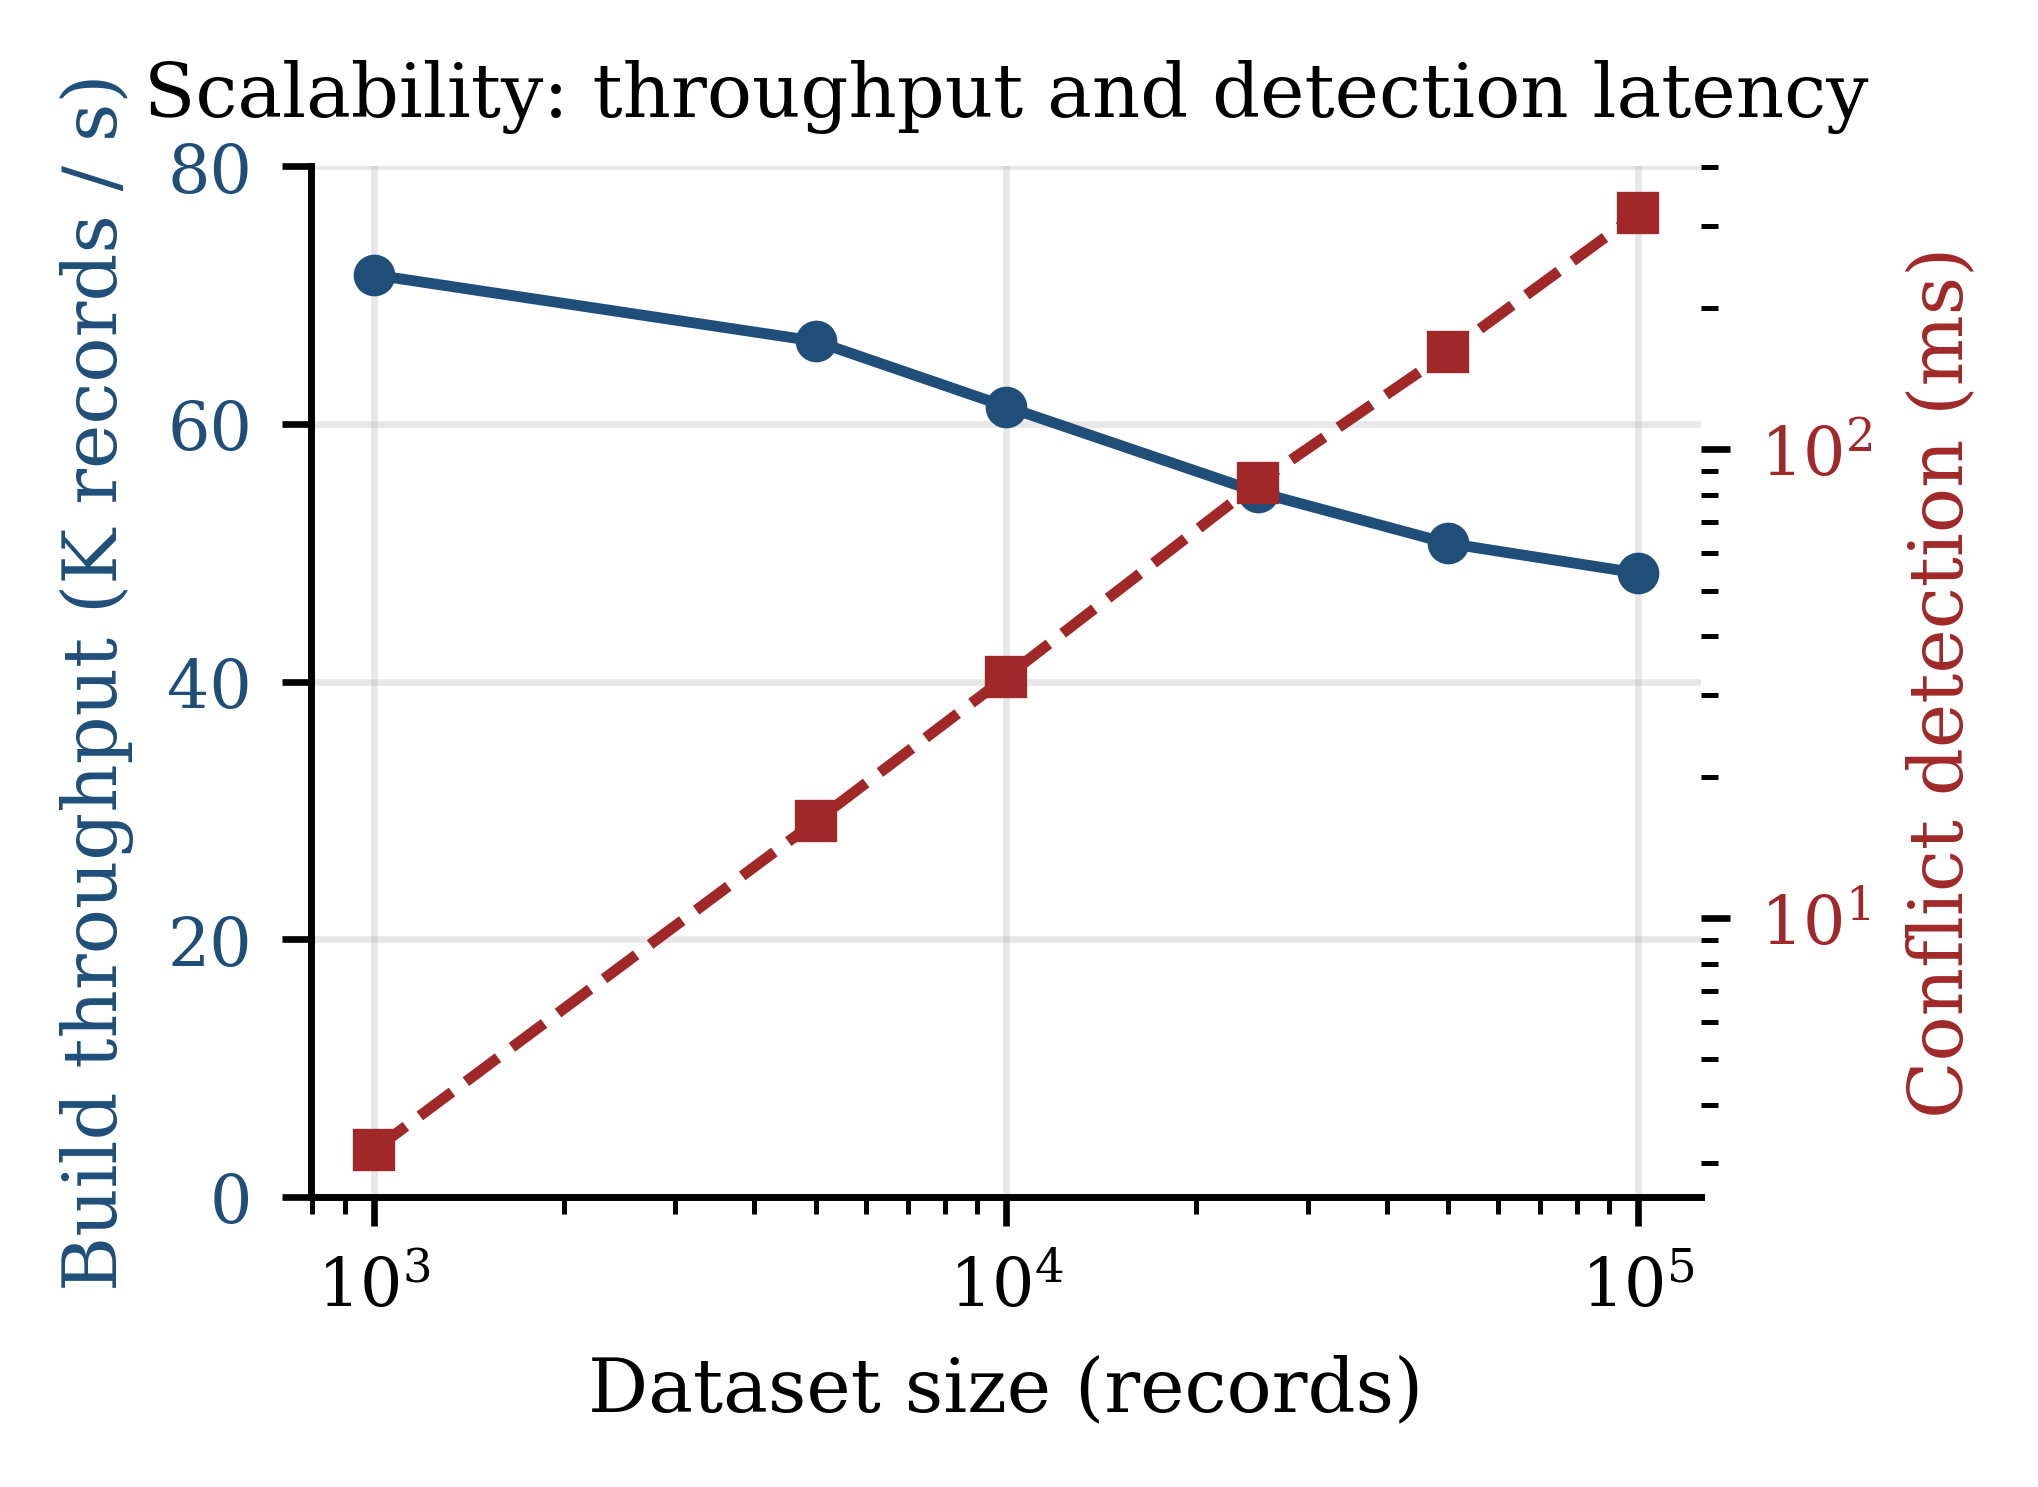
\includegraphics[width=\linewidth]{figures/fig4_scalability.png}
\caption{Build throughput (left axis, linear) and conflict-detection latency (right axis, log) versus dataset scale.}
\label{fig:scalability}
\end{figure}

The empirical conflict-detection time of $\approx 3.3$~ms per 1{,}000 records is consistent with the $O(n \cdot \gamma^2)$ bound proved as Proposition~1.

\subsection{Governance Scenarios}

Three end-to-end governance scenarios are run on the 10K dataset across all ten seeds and reported as mean $\pm \sigma$ in Table~\ref{tab:scenarios}. Scenario~B uses EU-custodian-stratified seed selection (one EU custodian per seed) to keep the per-seed cohort small but identifiable.

\begin{table}[t]
\centering
\caption{End-to-end governance scenario results (10K dataset, 10 seeds).}
\label{tab:scenarios}
\begin{tabular}{p{0.95\linewidth}}
\hline\hline
\textbf{A: Cross-system legal hold.} $645 \pm 128$ seeds (custodian + date filter); $1{,}454 \pm 256$ records after Att + Thread propagation; $810 \pm 132$ additional records via cross-system links across 4 source systems. \\
\hline
\textbf{B: GDPR erasure request.} $19 \pm 11$ PII records (single EU-custodian stratification at \texttt{eu\_cust[0]}, 10K dataset); $16 \pm 7$ freely deletable; $4 \pm 8$ retention-blocked; $4 \pm 8$ carry an active regulatory conflict requiring legal review. The variance across seeds reflects the small per-seed cohort produced by the single-custodian stratification --- reported faithfully rather than masked by a multi-custodian average. \\
\hline
\textbf{C: Multi-jurisdiction financial audit.} 500 financial records; $416 \pm 52$ conflicts; $69 \pm 26$ at critical or high severity. \\
\hline\hline
\end{tabular}
\end{table}

\subsection{Ablation Study}

Table~\ref{tab:ablation} reports the ablation. The experiment uses 50 matter-scoped seeds at depth 10, so the Full T-RKG hold set of 154 (3.07$\times$) here corresponds directly to the Att + Thread row in Table~\ref{tab:propagation}.

\begin{table}[t]
\centering
\caption{Ablation study (10K dataset, 50 matter-scoped seeds, depth 10, 10 seeds).}
\label{tab:ablation}
\begin{tabular}{lccccr}
\hline\hline
Variant & Ont. & Typed & Prop. & Conflicts & Hold set \\
\hline
Full T-RKG       & \checkmark & \checkmark & \checkmark & $740 \pm 89$    & 154 (3.07$\times$) \\
No Ontology      & ---        & \checkmark & \checkmark & $1{,}500 \pm 0$ (det.) & 154 (3.07$\times$) \\
No Typed Rels    & \checkmark & ---        & \checkmark & $740 \pm 89$    & 214 (4.28$\times$) \\
No Propagation   & \checkmark & \checkmark & ---        & $740 \pm 89$    & 50 (1.00$\times$) \\
Siloed Baseline  & ---        & ---        & ---        & $573 \pm 106$   & 50 (1.00$\times$) \\
\hline\hline
\end{tabular}
\end{table}

\subsection{Performance vs.\ Flat and Relational Alternatives}

\begin{table}[t]
\centering
\caption{Performance comparison on identical 10K-record workloads (10 seeds).}
\label{tab:perf}
\begin{tabular}{lccc}
\hline\hline
Operation & T-RKG (ms) & Flat (ms) & SQLite (ms) \\
\hline
Type query                            & $1.54 \pm 0.15$  & $0.36 \pm 0.01$ & $0.79 \pm 0.03$ \\
Hold propagation (Att+Thread, $d{=}5$) & $0.27 \pm 0.08$ & $10.57 \pm 3.24$  & $47.22 \pm 14.46$ \\
Conflict detection                    & $32.32 \pm 0.41$ & n/a             & n/a \\
Temporal point-in-time query          & $0.28 \pm 0.05$  & $0.21 \pm 0.01$ & $1.40 \pm 0.12$ \\
\hline\hline
\end{tabular}
\end{table}

\begin{figure}[t]
\centering
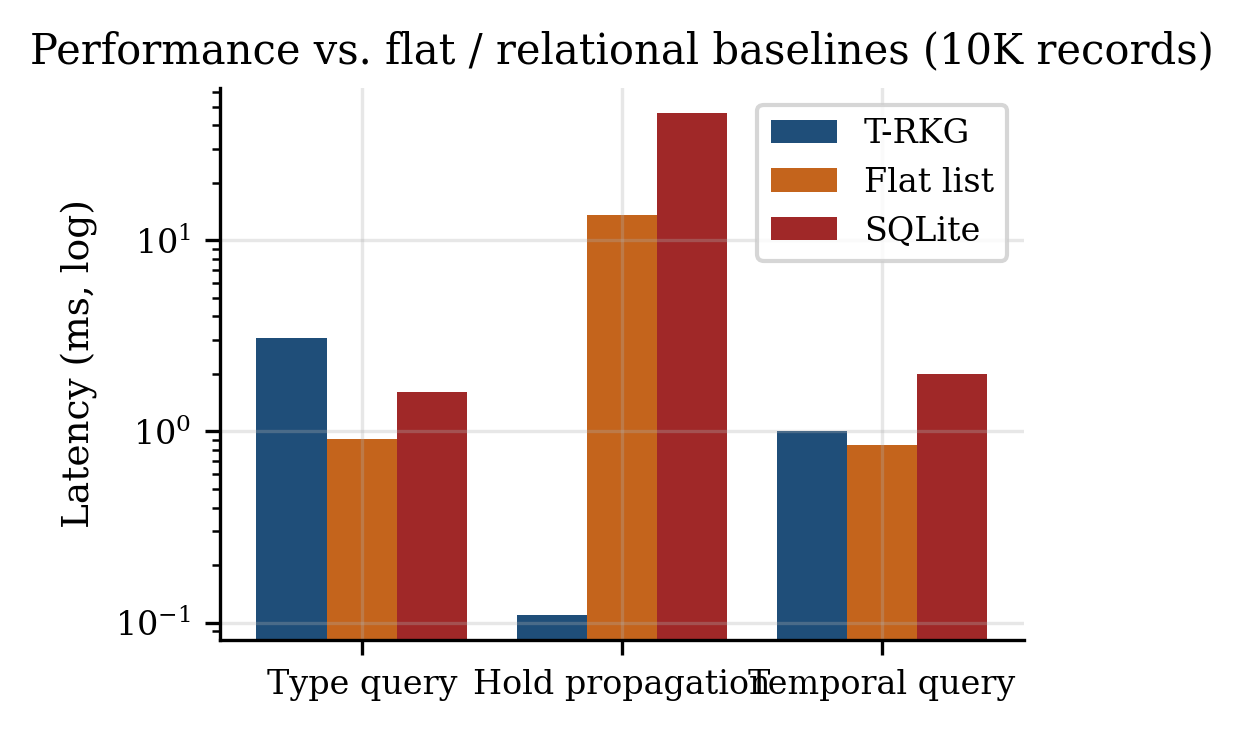
\includegraphics[width=\linewidth]{figures/fig9_perf_baselines.png}
\caption{Per-operation latency on identical 10K workloads (log scale). Propagation is the operation where graph-native indexing beats both alternatives by two-to-three orders of magnitude.}
\label{fig:perf}
\end{figure}

Hold propagation is the operation T-RKG's indexed adjacency lists were designed for. Type queries are slower in T-RKG than SQLite because the prototype iterates a Python dict without a type-keyed index — an implementation gap, not a structural finding. A comparison against production graph databases (Neo4j, Amazon Neptune, JanusGraph) is the natural next step and is left to follow-up work; the qualitative ranking (graph-native traversal beats relational recursive-CTE on hold propagation) is well-established in the graph-database literature and is not the contribution this paper claims novelty over.

\subsection{Propagation Latency vs.\ Seed-Set Size}

\begin{table}[t]
\centering
\caption{Propagation latency vs.\ seed set size on a 100K-record corpus (depth 5, 10 seeds). Largest reported seed set is 5K; behavior beyond this range is not measured.}
\label{tab:largeseed}
\begin{tabular}{rccr}
\hline\hline
Seed records & Latency (ms) & Hold set size & Per-seed cost \\
\hline
50    & $0.37 \pm 0.09$ & $97 \pm 19$    & 7.4~$\mu$s \\
500   & $2.80 \pm 0.21$  & $884 \pm 54$    & 5.6~$\mu$s \\
5{,}000 & $24.89 \pm 0.52$  & $8{,}342 \pm 119$  & 5.0~$\mu$s \\
\hline\hline
\end{tabular}
\end{table}

\begin{figure}[t]
\centering
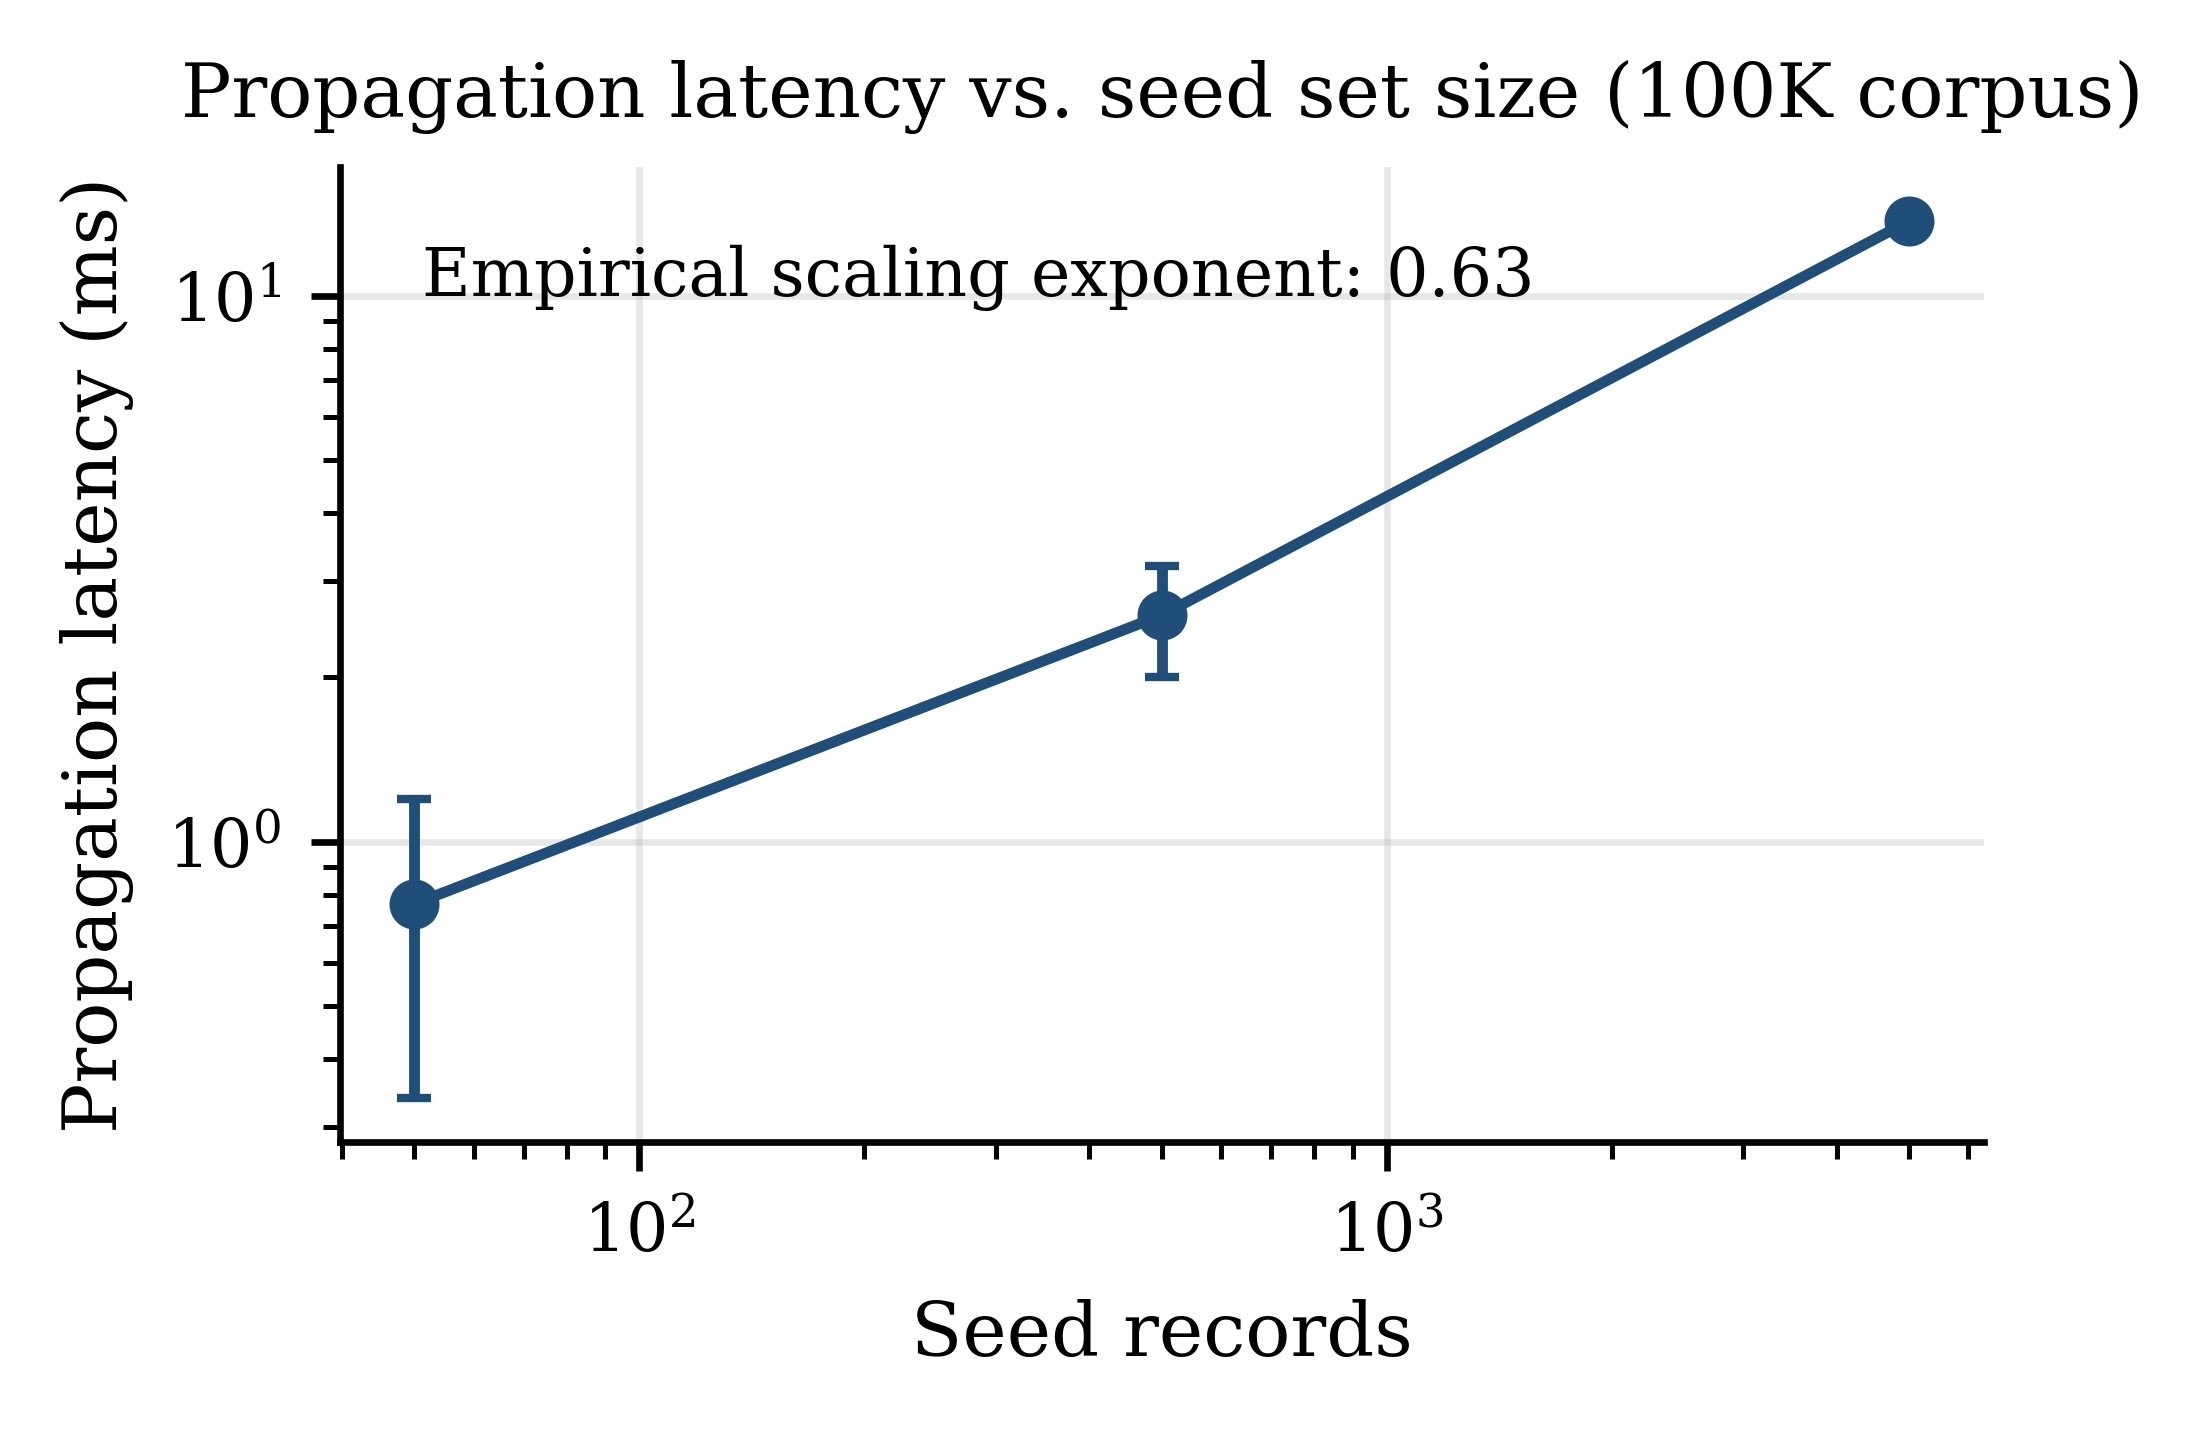
\includegraphics[width=\linewidth]{figures/fig6_propagation_vs_seeds.png}
\caption{Propagation latency versus seed set size on a 100K corpus (log-log).}
\label{fig:largeseed}
\end{figure}

Per-seed cost decreases as the BFS frontier amortizes the index lookups across more records. Empirical scaling exponent $\approx 0.87$ (sub-linear in seed count), consistent with the $O(|H| + |E_H|)$ bound of Proposition~2 once the connected component is saturated. We do not claim production-scale performance --- legal matters routinely exceed 50{,}000 custodians across millions of records and this regime is not within the in-memory implementation's range.

\subsection{GDPR Art.~17(3) Exemption Impact}
\label{sec:exemption}

Table~\ref{tab:exemption} reports the suppression effect of Axiom~4 under a controlled hold scenario. The per-seed protocol is:
\begin{enumerate}
    \item generate the 10K dataset; matters carry the \texttt{legal\_obligation} and \texttt{legal\_claim} flags sampled at $p{=}0.05$ each, independently;
    \item identify the EU+PII population --- the records GDPR Article~17 erasure attaches to;
    \item distribute holds round-robin across all five active matters;
    \item run the detector twice: once with the matter dictionary supplied (Axiom~4 active), once without (no suppression).
\end{enumerate}

\begin{table}[t]
\centering
\caption{Art.~17(3) exemption impact (10K dataset, 10 seeds, EU+PII cohort, hold distributed round-robin across 5 matters). Standard deviation reflects the integer realization of Bernoulli($p{=}0.05$) exemption flags across five matters per seed (expected number of exempted matters per seed $\approx 0.49$); this is a sampling-design artifact, not measurement instability.}
\label{tab:exemption}
\begin{tabular}{lc}
\hline\hline
Measurement & Mean $\pm \sigma$ \\
\hline
EU+PII records held                              & $395 \pm 60$ \\
Hold-Deletion conflicts (no suppression)         & $395 \pm 60$ \\
Hold-Deletion conflicts (Axiom~4 active)         & $353 \pm 59$ \\
Suppressed by Art.~17(3) exemption               & $42 \pm 44$  \\
Suppression rate                                 & $\sim$10.5\%    \\
\hline\hline
\end{tabular}
\end{table}

The suppression-rate variance ($42 \pm 44$) is dominated by the discrete distribution of exempted matters. With five matters and two independent Bernoulli($0.05$) flags per matter, the expected fraction of exempted matters is $1{-}(1{-}0.05)^2 \approx 0.0975$. At the single-dataset scale this rounds to $0/5$, $1/5$, or $2/5$ matters per seed; across the ten seeds the obligation flag landed on a single matter in 2 of 10 runs and the claim flag landed on a single matter in 3 of 10 runs, with no seed producing two exempted matters under the same flag. The mean suppression rate matches the population-level expectation; the wide standard deviation is what those small integer counts produce on a ten-seed sample. A continuous-rate sampling design would yield a tighter band but would no longer reflect the integer realization of the matter-level encoding, which is the encoding faithful to the regulatory text.

\subsection{Robustness to Synthetic-Data Parameters}
\label{sec:robustness}

Table~\ref{tab:robustness} sweeps the two parameters most likely to vary across organizations: the EU jurisdictional fraction (5\% to 40\%) and the PII rate (5\%, 20\%).

\begin{table}[t]
\centering
\caption{Robustness to jurisdictional mix $\times$ PII rate (10K dataset, 10 seeds).}
\label{tab:robustness}
\begin{tabular}{ccccc}
\hline\hline
EU frac & PII rate & Total conflicts & Cross-domain & Multi-reg \\
\hline
5\%  & 5\%  & $423 \pm 79$ & $41 \pm 25$  & $224 \pm 32$ \\
5\%  & 20\% & $423 \pm 79$ & $41 \pm 25$  & $225 \pm 32$ \\
15\% & 5\%  & $466 \pm 80$ & $84 \pm 36$  & $256 \pm 38$ \\
15\% & 20\% & $466 \pm 80$ & $84 \pm 36$  & $257 \pm 38$ \\
30\% & 5\%  & $443 \pm 93$ & $119 \pm 47$ & $269 \pm 52$ \\
30\% & 20\% & $443 \pm 93$ & $119 \pm 47$ & $270 \pm 52$ \\
40\% & 5\%  & $429 \pm 96$ & $141 \pm 38$ & $276 \pm 51$ \\
40\% & 20\% & $429 \pm 96$ & $141 \pm 38$ & $277 \pm 51$ \\
\hline\hline
\end{tabular}
\end{table}

\begin{figure}[t]
\centering
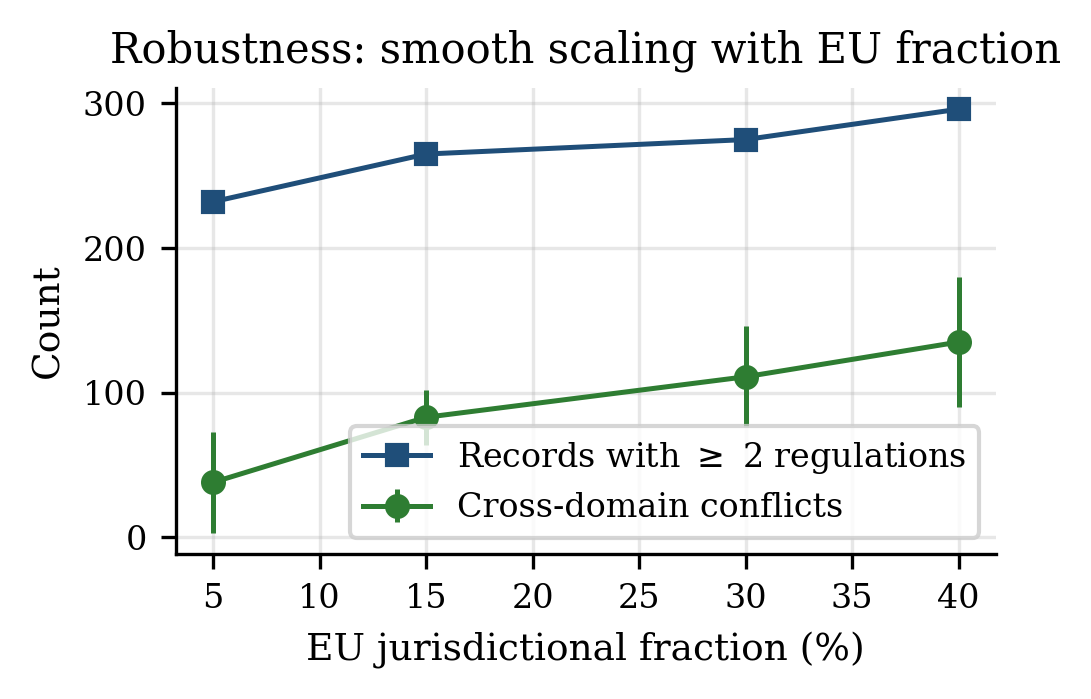
\includegraphics[width=\linewidth]{figures/fig7_robustness_sweep.png}
\caption{Cross-domain conflicts and multi-regulation record counts as the EU jurisdictional fraction increases. No discontinuities are observed.}
\label{fig:robustness}
\end{figure}

Cross-domain conflict count varies smoothly and roughly monotonically with EU fraction across the swept range. The smooth gradient is consistent with the synthetic-data methodology but is not evidence that the same gradient would hold on a production corpus with non-i.i.d.\ jurisdictional structure.

\subsection{Reproduction}
\label{sec:repro}

All reported numbers are produced by a single command: \texttt{python -m experiments.run\_all}. Expected runtime is 60 to 180 seconds on commodity hardware (the SHACL baseline contributes most of that; the original eleven experiments run in 30--90 seconds). Absolute wall-clock times will vary by a few percent across hardware, but the distributions reproduce under the documented ten-seed set. Outputs land in \texttt{experiments/results.json}. The OWL ontology parses with any conformant OWL~2 / RDF Turtle tool (\texttt{python -c "import rdflib; rdflib.Graph().parse('ontology/trkg.ttl', format='turtle')"}; the \texttt{owlready2} parser requires the file-extension hint). The supplementary repository includes a unit-test suite covering the ontology, conflict detector, baselines (including the SHACL Core and SHACL-SPARQL baselines), the Art.~17(3) exemption logic, the cross-system partition, and the competency questions. The LLM baseline of §\ref{sec:llm} is reproduced from a cached set of model responses shipped with the supplementary code, so the reported figures replay deterministically; re-querying the model live requires an API key and will incur minor per-call variation in wording but not in the scored applicability sets.

\textit{Encoding-validation note.} During pre-submission validation of the applicability encoding against the ontology's own class hierarchy and against independent expert labeling (§\ref{sec:expert}), three encoding refinements were applied. First, the SEC profile was not gated on public-company status, so it could fire on private-company financial records; it is now gated consistently with the SOX profile. Second, the financial-regulation profiles (SOX, SEC, IRS, and the German HGB) did not reflect the ontology's declared subclass relationships, under which \texttt{TaxRecord} and \texttt{AuditWorkpaper} are subclasses of \texttt{FinancialRecord} (\texttt{trkg.ttl}); these record types now inherit the applicable financial-regulation profiles. Third, the FINRA profile had been extended to all financial-family record types by that same inheritance, but FINRA Rule~4511 is scoped to broker-dealer member firms' books and records rather than to financial records generally; its record-type set was therefore narrowed to business communications (email and chat retained under Rule~4511 / SEC Rule~17a-4). All counts reported in this paper reflect the corrected encoding. The first two corrections increase total conflict counts on tax-record-heavy datasets (the previous encoding under-counted); the FINRA narrowing affects only per-regulation applicability counts, not conflict counts (FINRA participates in no pairwise conflict rule). The clean-regime applicability identity and the qualitative baseline orderings are unchanged.

\section{Discussion}

\subsection{Interpreting the Experimental Record}

The cross-domain conflict comparison is best understood as empirical confirmation of Corollary~1, not as a head-to-head between competing implementations. The corollary proves that an attribute-blind tagging baseline cannot detect the cross-domain conflicts T-RKG detects; the ``0~$\pm$~0'' baseline numbers in Table~\ref{tab:conflicts} are what that proof predicts, not an independent measurement. The empirical weight of the evaluation rests instead on three results that are not forced by construction: the composition ablation (§\ref{sec:composition}), in which removing cross-system composition while holding the ontology and regulation set fixed collapses cross-domain detection to zero on every seed; the noise-robustness of applicability reasoning (Table~\ref{tab:f1noise}), with T-RKG at F1 $0.826 \pm 0.011$ under 10\% corruption; and the LLM baseline (§\ref{sec:llm}), which shows that even a capable model cannot detect cross-domain conflicts from a siloed view, isolating composition rather than classification as the operative difficulty. The propagation results carry larger variance, reflecting structural variation in matter-level relationship density across seeds rather than algorithmic instability.

\subsection{Architectural Tradeoffs}

T-RKG is implemented as a metadata-extraction layer for a practical reason: relocating enterprise document stores is operationally infeasible at most organizations of the scale this work targets. Extracting only relationship metadata and governance-relevant record attributes allows incremental deployment alongside existing source systems. The architecture does not address connector maintenance, which scales with the number of source systems and changes with each platform release.

\subsection{The Composite-Record Distinction in Practice}

The composite-record formulation (§III-C) is the structural difference between T-RKG and the commercial governance products it is meant to complement, not replace. Most enterprise records-governance tooling is content-centric: rules attach to file type, container, or classification tag. The cross-domain conflicts reported in §VII-D are conflicts over records whose triggering attributes (PII flag, public-company flag, EU jurisdiction) live in different source systems and only co-occur after composition. T-RKG's ontology builds the composite explicitly; the applicability predicate runs over the composite; the cross-domain conflicts the evaluation surfaces would not be visible to any tooling that defines the record as content alone.

\subsection{Regulatory Scope and Extensibility}

The nine-regulation ontology covers the frameworks most commonly applicable to US-headquartered multinationals with European and Canadian operations. Extending the ontology to a new regulation requires authoring one applicability profile and encoding pairwise conflict rules against the existing set. Regulations whose applicability depends on industry-specific exemptions, evolving enforcement guidance, or contested jurisdictional boundaries require materially more effort and should involve domain experts in the encoding process. The Art.~17(3)(b) legal-obligation and Art.~17(3)(e) legal-claim exemptions are now encoded as Axiom~4 (§IV-E, evaluated in §VII-K); the three remaining §17(3) clauses --- (a) freedom of expression and information, (c) public-health processing, and (d) archiving in the public interest, scientific or historical research, and statistical purposes --- have not been encoded because each is conditioned on usage-context predicates (purpose-of-processing classifications) that are not currently materialized in the synthetic ABox. Adding them is straightforward once those predicates are added.

\subsection{Limitations}

\textit{Synthetic data.} The evaluation is entirely synthetic. The author's industry access did not permit even an anonymized single-matter validation within the submission timeline; this is the most consequential limitation of the present work and the primary target of follow-up. The generator's distributions are chosen as a plausible enterprise prior; Table~\ref{tab:robustness} shows that conflict counts vary smoothly with the two parameters most likely to differ across organizations, but production deployments will encounter organizational specifics the generator does not anticipate.

\textit{Independent validation of the applicability predicate.}
\label{sec:expert}
Because the F1 results of §\ref{sec:f1} score T-RKG against a clean-label snapshot of its own regulation-assignment function, they measure robustness under corruption rather than agreement with an external standard. To check the encoded predicate against independent judgment, a stratified sample of 146 records from the synthetic corpus---spanning all nine regulations and balanced across the privacy, financial, and cross-domain trigger families---was labeled with the regulations judged applicable from each record's attributes, without sight of T-RKG's output. Agreement between the independent labels and T-RKG's predicate is high: across the $146 \times 9$ record--regulation cells, the two agree on 98.2\%. Per-regulation agreement is exact for the attribute-gated privacy and health regulations (GDPR, CPRA, PIPEDA, HIPAA) and for SOX; the small residual disagreements concentrate on the financial-overlay regulations (IRS, HGB, SEC), where applicability depends on the interaction of record type, public-company status, and US jurisdiction. This validation surfaced one encoding refinement---an over-broad FINRA record-type scope inherited from the financial-record class hierarchy, since narrowed to the broker-dealer communications FINRA Rule~4511 actually governs (§\ref{sec:repro}). The validation is against synthetic records and is not a substitute for evaluation on a production corpus, which remains the primary target of follow-up; it establishes that the encoded predicate matches independent judgment on the modeled attribute combinations.

\textit{Production graph database comparison.} Table~\ref{tab:perf} compares T-RKG against flat-list and SQLite alternatives. It does not compare against Neo4j, Amazon Neptune, or JanusGraph. The qualitative conclusion (graph-native traversal beats relational-CTE on hold propagation) is not expected to flip on those platforms; absolute numbers will reshape.

\textit{Noise model.} The §VII-B noised regime uses independent per-attribute label flips. Real source-system corruption is correlated and biased: a single bad ingestion run flips an entire batch, jurisdiction confusion follows administrative geography, missing-PII-flag dominates wrong-PII-flag. §VII-B reports a block-correlated companion experiment that partially addresses this, but it is not a substitute for production-data evaluation.

\textit{Ontology coverage.} Fourteen pairwise conflict rules across nine regulations represent a subset of the US-global compliance space. FERPA, CIPA, FINRA Rule~4511 in its granular detail, and the EU AI Act's data-governance provisions are not included.

\textit{Explicit relationship assumption.} T-RKG reasons over relationships that source systems have formally recorded. Implicit or semantic relationships between records are outside the system's current scope.

\textit{Single-jurisdiction record assignment.} The default generator assigns each record a single primary jurisdiction, under which the Jurisdiction conflict family (GDPR vs.\ CPRA, GDPR vs.\ PIPEDA) cannot fire, since those pairs require a record subject to two privacy regimes at once. To demonstrate that the family is reachable, a capability-coverage experiment (§\ref{sec:robustness}) uses an optional multi-jurisdiction representation in which a record may carry additional jurisdictions; under that representation all four conflict families fire. This is a deliberate extension exercised only in the coverage experiment, not the default generator; production deployments would encounter multi-jurisdiction records at organization-specific rates the synthetic prior does not attempt to fix.

\textit{Bitemporal evaluation.} §V-E names the bitemporal model but the evaluation in §VII exercises only the valid-time axis; a transaction-time experiment is roadmap work.

\section{Conclusion}

The composite-record formulation, expressed as ontology-driven applicability inference over typed temporal relationships, makes cross-system regulatory conflicts visible at a cost of roughly 320~ms per 100K records on a single host. Corollary~1 explains why the two ablation baselines return zero cross-domain conflicts: under attribute-blind tagging the conflicts are not detectable in principle, so the baseline numbers do not themselves quantify T-RKG's advantage. The contribution rests on what survives that disclaimer. The noised-regime F1 of $0.826 \pm 0.011$ separates T-RKG from the Siloed ($0.604 \pm 0.035$) and No-Ontology ($0.141 \pm 0.011$) baselines under 10\% per-attribute label noise. The SHACL Core baseline detects roughly 4\% of T-RKG's conflicts at 100K records and takes about $62\times$ longer to do so, with the rule families it cannot express catalogued in the supplementary material against their specification gaps. The contribution would be falsified by a production-graph-DB implementation of the same ontology that reverses the latency ranking, or by a real-corpus evaluation in which the noised-regime F1 falls below the Siloed baseline. Open items: encoding the Art.~17(3) clauses (a), (c), and (d) once purpose-of-processing predicates are materialized; a structured-noise evaluation regime; and partner-tenant integration against a real enterprise corpus.

\section*{Acknowledgment}

The author used an AI assistant for sentence-level editing on portions of the manuscript and for implementation assistance on parts of the rule-evaluation logic in \texttt{trkg/conflict.py} and the plotting code in \texttt{figures/make\_figures.py}. All experimental design, ontology authoring, axiom derivation, statistical methodology, interpretation of results, and contribution claims are the author's. AI-generated code was reviewed and integrated only after passing the unit tests in \texttt{tests/}. AI-edited prose was revised by the author. No external funding supported this work. The views expressed are the author's own and do not necessarily represent those of any affiliated organization.

\begin{thebibliography}{50}

\bibitem{edrm}
EDRM, ``Electronic Discovery Reference Model,'' 2020. [Online]. Available: \url{https://edrm.net}

\bibitem{iso15489}
ISO, ``ISO 15489-1:2016 Information and Documentation: Records Management,'' International Organization for Standardization, 2016.

\bibitem{sergot1986}
M.~J.~Sergot, F.~Sadri, R.~A.~Kowalski, F.~Kriwaczek, P.~Hammond, and H.~T.~Cory, ``The British Nationality Act as a Logic Program,'' \textit{Communications of the ACM}, vol.~29, no.~5, pp.~370--386, 1986.

\bibitem{ashley2017}
K.~D.~Ashley, \textit{Artificial Intelligence and Legal Analytics: New Tools for Law Practice in the Digital Age}. Cambridge University Press, 2017.

\bibitem{legalruleml}
M.~Palmirani, G.~Governatori, A.~Rotolo, S.~Tabet, H.~Boley, and A.~Paschke, ``LegalRuleML: XML-Based Rules and Norms,'' in \textit{Proc. RuleML}, LNCS 7018, Springer, 2011, pp.~298--312.

\bibitem{lkif}
R.~Hoekstra, J.~Breuker, M.~Di Bello, and A.~Boer, ``The LKIF Core Ontology of Basic Legal Concepts,'' in \textit{Proc. LOAIT Workshop}, 2007, pp.~43--63.

\bibitem{gdprpcikg}
L.~Elluri, A.~Nagar, and K.~P.~Joshi, ``An Integrated Knowledge Graph to Automate GDPR and PCI DSS Compliance,'' in \textit{Proc. IEEE Int. Conf. Big Data (Big Data)}, 2018, pp.~1266--1271.

\bibitem{compliancenlp}
D.~Guo, J.~Wu, and S.~M.~Yiu, ``ComplianceNLP: Knowledge-Graph-Augmented RAG for Multi-Framework Regulatory Gap Detection,'' arXiv:2604.23585, 2026.

\bibitem{graphcompliance}
J.~Chung, R.~Ko, W.~Yoo, M.~Onizuka, S.~Kim, T.~Kim, and W.~Shin, ``GraphCompliance: Aligning Policy and Context Graphs for LLM-Based Regulatory Compliance,'' arXiv:2510.26309, 2025.

\bibitem{conflictnorms}
L.~Robaldo, S.~Batsakis, R.~Calegari, F.~Calimeri, M.~Fujita, G.~Governatori, M.~C.~Morelli, F.~Pacenza, G.~Pisano, K.~Satoh, I.~Tachmazidis, and J.~Zangari, ``Compliance Checking on First-Order Knowledge with Conflicting and Compensatory Norms: A Comparison Among Currently Available Technologies,'' \textit{Artificial Intelligence and Law}, vol.~32, no.~2, pp.~505--555, 2024.

\bibitem{ragulating}
B.~Agarwal, H.~S.~Jomraj, S.~Kaplunov, J.~Krolick, and V.~Rojkova, ``RAGulating Compliance: A Multi-Agent Knowledge Graph for Regulatory QA,'' arXiv:2508.09893, 2025.

\bibitem{privcompkg}
L.~Garza, L.~Elluri, A.~Piplai, A.~Kotal, D.~Gupta, and A.~Joshi, ``PrivComp-KG: Leveraging Knowledge Graph and Large Language Models for Privacy Policy Compliance Verification,'' arXiv:2404.19744, 2024.

\bibitem{akomantoso}
OASIS LegalDocML TC, ``Akoma Ntoso Version 1.0,'' OASIS Standard, 27~Aug.~2018.

\bibitem{governatori2013}
G.~Governatori, F.~Olivieri, A.~Rotolo, and S.~Scannapieco, ``Computing Strong and Weak Permissions in Defeasible Logic,'' \textit{Journal of Philosophical Logic}, vol.~42, no.~6, pp.~799--829, 2013.

\bibitem{weber2019}
M.~Weber \textit{et al.}, ``Anti-Money Laundering in Bitcoin: Experimenting with Graph Convolutional Networks for Financial Forensics,'' in \textit{Proc. KDD Workshop on Anomaly Detection in Finance}, 2019.

\bibitem{fibo}
EDM Council, ``Financial Industry Business Ontology (FIBO),'' Specification, ongoing maintenance, 2013--2026.

\bibitem{arner2017}
D.~W.~Arner, J.~Barberis, and R.~P.~Buckley, ``FinTech, RegTech, and the Reconceptualization of Financial Regulation,'' \textit{Northwestern Journal of International Law and Business}, vol.~37, no.~3, pp.~371--413, 2017.

\bibitem{legalbert}
I.~Chalkidis \textit{et al.}, ``LEGAL-BERT: The Muppets Straight out of Law School,'' in \textit{Findings of EMNLP}, 2020, pp.~2898--2904.

\bibitem{galkin2017}
M.~Galkin, S.~Auer, M.-E.~Vidal, and S.~Scerri, ``Enterprise Knowledge Graphs: A Semantic Approach for Knowledge Management in the Next Generation of Enterprise Information Systems,'' in \textit{Proc. ICEIS}, vol.~2, 2017, pp.~88--98.

\bibitem{noy2019}
N.~Noy, Y.~Gao, A.~Jain, A.~Narang, A.~Patterson, and J.~Taylor, ``Industry-Scale Knowledge Graphs: Lessons and Challenges,'' \textit{Communications of the ACM}, vol.~62, no.~8, pp.~36--43, 2019.

\bibitem{pan2024}
S.~Pan, L.~Luo, Y.~Wang, C.~Chen, J.~Wang, and X.~Wu, ``Unifying Large Language Models and Knowledge Graphs: A Roadmap,'' \textit{IEEE Trans. Knowledge and Data Engineering}, vol.~36, no.~7, pp.~3580--3599, 2024.

\bibitem{purview}
Microsoft, ``Microsoft Purview Documentation,'' Microsoft Learn, 2024. [Online]. Available: \url{https://learn.microsoft.com/en-us/purview/}. Accessed: 2026-05-25.

\bibitem{odrl}
R.~Iannella and S.~Villata (eds.), ``ODRL Information Model 2.2,'' W3C Recommendation, 15~Feb.~2018.

\bibitem{gutierrez2007}
C.~Gutierrez, C.~A.~Hurtado, and A.~Vaisman, ``Introducing Time into RDF,'' \textit{IEEE Trans. Knowledge and Data Engineering}, vol.~19, no.~2, pp.~207--218, 2007.

\bibitem{allen1983}
J.~F.~Allen, ``Maintaining Knowledge about Temporal Intervals,'' \textit{Communications of the ACM}, vol.~26, no.~11, pp.~832--843, 1983.

\bibitem{snodgrass1995}
R.~T.~Snodgrass (ed.), \textit{The TSQL2 Temporal Query Language}. Kluwer Academic, 1995.

\bibitem{jensen1997}
J.~Clifford, C.~E.~Dyreson, T.~Isakowitz, C.~S.~Jensen, and R.~T.~Snodgrass, ``On the Semantics of `Now' in Databases,'' \textit{ACM Trans.\ Database Systems}, vol.~22, no.~2, pp.~171--214, 1997.

\bibitem{transe}
A.~Bordes, N.~Usunier, A.~Garcia-Duran, J.~Weston, and O.~Yakhnenko, ``Translating Embeddings for Modeling Multi-relational Data,'' in \textit{Proc. NeurIPS}, 2013.

\bibitem{rotate}
Z.~Sun, Z.~Deng, J.-Y.~Nie, and J.~Tang, ``RotatE: Knowledge Graph Embedding by Relational Rotation in Complex Space,'' in \textit{Proc. ICLR}, 2019.

\bibitem{timeplex}
P.~Jain, S.~Rathi, and S.~Chakrabarti, ``Temporal Knowledge Base Completion: New Algorithms and Evaluation Protocols,'' in \textit{Proc. EMNLP}, 2020.

\bibitem{tlogic}
Y.~Liu, Y.~Ma, M.~Hildebrandt, M.~Joblin, and V.~Tresp, ``TLogic: Temporal Logical Rules for Explainable Link Forecasting on Temporal Knowledge Graphs,'' in \textit{Proc. AAAI}, 2022.

\bibitem{temp}
J.~Wu, M.~Cao, J.-K.~Cheung, and W.~Hamilton, ``TeMP: Temporal Message Passing for Temporal Knowledge Graph Completion,'' in \textit{Proc. EMNLP}, 2020.

\bibitem{tie}
Z.~Han, P.~Chen, Y.~Ma, and V.~Tresp, ``TIE: A Framework for Embedding-based Incremental Temporal Knowledge Graph Completion,'' in \textit{Proc. ACL}, 2021.

\bibitem{cai2023}
H.~Cai, Y.~Liao, and R.~Li, ``Temporal Knowledge Graph Completion: A Survey,'' arXiv:2308.02457, 2023.

\bibitem{cai2024tkgsurvey}
L.~Cai, X.~Mao, Y.~Zhou, Z.~Long, C.~Wu, and M.~Lan, ``A Survey on Temporal Knowledge Graph: Representation Learning and Applications,'' arXiv:2403.04782, 2024.

\bibitem{gruber1995}
T.~R.~Gruber, ``Toward Principles for the Design of Ontologies Used for Knowledge Sharing,'' \textit{International Journal of Human-Computer Studies}, vol.~43, no.~5--6, pp.~907--928, 1995.

\bibitem{guarino2009}
N.~Guarino, D.~Oberle, and S.~Staab, ``What is an Ontology?'' in \textit{Handbook on Ontologies}, 2nd ed. Springer, 2009.

\bibitem{uschold1998}
M.~Uschold, M.~King, S.~Moralee, and Y.~Zorgios, ``The Enterprise Ontology,'' \textit{Knowledge Engineering Review}, vol.~13, no.~1, pp.~31--89, 1998.

\bibitem{gruninger1995}
M.~Gr\"{u}ninger and M.~S.~Fox, ``The Role of Competency Questions in Enterprise Ontology Design,'' in \textit{Benchmarking: Theory and Practice}, Springer, 1995.

\bibitem{schriml2019}
L.~M.~Schriml \textit{et al.}, ``Human Disease Ontology 2018 Update: Classification, Content and Workflow Expansion,'' \textit{Nucleic Acids Research}, vol.~47, no.~D1, pp.~D955--D962, 2019.

\bibitem{ringsquandl2015}
M.~Ringsquandl, S.~Lamparter, S.~Brandt, T.~Hubauer, and R.~Lepratti, ``Semantic-Guided Feature Selection for Industrial Automation Systems,'' in \textit{The Semantic Web (ISWC 2015)}, LNCS 9366, Springer, 2015, pp.~225--240.

\bibitem{pygraft}
N.~Hubert, P.~Monnin, M.~d'Aquin, D.~Monticolo, and A.~Brun, ``PyGraft: Configurable Generation of Synthetic Schemas and Knowledge Graphs at Your Fingertips,'' in \textit{Proc. ESWC}, 2024.

\bibitem{vanderaalst2016}
W.~M.~P.~van der Aalst, \textit{Process Mining: Data Science in Action}, 2nd ed. Springer, 2016.

\bibitem{networkx}
A.~A.~Hagberg, D.~A.~Schult, and P.~J.~Swart, ``Exploring Network Structure with NetworkX,'' in \textit{Proc. SciPy}, 2008.

\bibitem{hogan2021}
A.~Hogan \textit{et al.}, ``Knowledge Graphs,'' \textit{ACM Computing Surveys}, vol.~54, no.~4, Art.~71, 2021.

\bibitem{bizer2009}
C.~Bizer, T.~Heath, and T.~Berners-Lee, ``Linked Data: The Story So Far,'' \textit{International Journal on Semantic Web and Information Systems}, vol.~5, no.~3, 2009.

\bibitem{brank2005}
J.~Brank, M.~Grobelnik, and D.~Mladeni\'{c}, ``A Survey of Ontology Evaluation Techniques,'' in \textit{Proc. SiKDD}, 2005.

\bibitem{shacl}
H.~Knublauch and D.~Kontokostas, ``Shapes Constraint Language (SHACL),'' W3C Recommendation, 2017.

\bibitem{owl2}
B.~Motik \textit{et al.}, ``OWL 2 Web Ontology Language Profiles,'' W3C Recommendation, 2nd ed., 2012.


\bibitem{sparql}
E.~Prud'hommeaux and A.~Seaborne (eds.), ``SPARQL Query Language for RDF,'' W3C Recommendation, 2008.

\bibitem{linkeddata}
T.~Berners-Lee, ``Linked Data: Design Issues,'' W3C Personal Note, 2006/2009.

\bibitem{antoniou2012}
G.~Antoniou and F.~van Harmelen, \textit{A Semantic Web Primer}, 3rd ed. MIT Press, 2012.

\end{thebibliography}

\begin{IEEEbiographynophoto}{KISHORE PULAGAM}
received the B.Tech.\ degree in Electronics and Communication Engineering from JNTU Hyderabad, India, in 2008, and the M.Sc.\ degree in Computer Networks from Middlesex University, London, U.K., in 2010. He is currently pursuing the Executive M.B.A.\ degree at the Kellogg School of Management, Northwestern University, Evanston, IL, USA.

He is a Senior Staff Software Engineer at PayPal, where he serves as the technical lead for enterprise content management and AI-powered document intelligence systems deployed at global scale. He has more than a decade of experience architecting and deploying production-scale information retrieval and machine learning infrastructure, including distributed FAISS vector databases, retrieval-augmented generation pipelines, and large language model based document classification services. His research interests include information retrieval, knowledge graphs, document understanding, and information governance for AI systems in regulated environments. His current research focuses on knowledge-based systems for cross-system regulatory governance.
\end{IEEEbiographynophoto}

\EOD

\end{document}
